\documentclass[1p]{elsarticle_modified}
%\bibliographystyle{elsarticle-num}

%\usepackage[colorlinks]{hyperref}
%\usepackage{abbrmath_seonhwa} %\Abb, \Ascr, \Acal ,\Abf, \Afrak
\usepackage{amsfonts}
\usepackage{amssymb}
\usepackage{amsmath}
\usepackage{amsthm}
\usepackage{scalefnt}
\usepackage{amsbsy}
\usepackage{kotex}
\usepackage{caption}
\usepackage{subfig}
\usepackage{color}
\usepackage{graphicx}
\usepackage{xcolor} %% white, black, red, green, blue, cyan, magenta, yellow
\usepackage{float}
\usepackage{setspace}
\usepackage{hyperref}

\usepackage{tikz}
\usetikzlibrary{arrows}

\usepackage{multirow}
\usepackage{array} % fixed length table
\usepackage{hhline}

%%%%%%%%%%%%%%%%%%%%%
\makeatletter
\renewcommand*\env@matrix[1][\arraystretch]{%
	\edef\arraystretch{#1}%
	\hskip -\arraycolsep
	\let\@ifnextchar\new@ifnextchar
	\array{*\c@MaxMatrixCols c}}
\makeatother %https://tex.stackexchange.com/questions/14071/how-can-i-increase-the-line-spacing-in-a-matrix
%%%%%%%%%%%%%%%

\usepackage[normalem]{ulem}

\newcommand{\msout}[1]{\ifmmode\text{\sout{\ensuremath{#1}}}\else\sout{#1}\fi}
%SOURCE: \msout is \stkout macro in https://tex.stackexchange.com/questions/20609/strikeout-in-math-mode

\newcommand{\cancel}[1]{
	\ifmmode
	{\color{red}\msout{#1}}
	\else
	{\color{red}\sout{#1}}
	\fi
}

\newcommand{\add}[1]{
	{\color{blue}\uwave{#1}}
}

\newcommand{\replace}[2]{
	\ifmmode
	{\color{red}\msout{#1}}{\color{blue}\uwave{#2}}
	\else
	{\color{red}\sout{#1}}{\color{blue}\uwave{#2}}
	\fi
}

\newcommand{\Sol}{\mathcal{S}} %segment
\newcommand{\D}{D} %diagram
\newcommand{\A}{\mathcal{A}} %arc


%%%%%%%%%%%%%%%%%%%%%%%%%%%%%5 test

\def\sl{\operatorname{\textup{SL}}(2,\Cbb)}
\def\psl{\operatorname{\textup{PSL}}(2,\Cbb)}
\def\quan{\mkern 1mu \triangleright \mkern 1mu}

\theoremstyle{definition}
\newtheorem{thm}{Theorem}[section]
\newtheorem{prop}[thm]{Proposition}
\newtheorem{lem}[thm]{Lemma}
\newtheorem{ques}[thm]{Question}
\newtheorem{cor}[thm]{Corollary}
\newtheorem{defn}[thm]{Definition}
\newtheorem{exam}[thm]{Example}
\newtheorem{rmk}[thm]{Remark}
\newtheorem{alg}[thm]{Algorithm}

\newcommand{\I}{\sqrt{-1}}
\begin{document}

%\begin{frontmatter}
%
%\title{Boundary parabolic representations of knots up to 8 crossings}
%
%%% Group authors per affiliation:
%\author{Yunhi Cho} 
%\address{Department of Mathematics, University of Seoul, Seoul, Korea}
%\ead{yhcho@uos.ac.kr}
%
%
%\author{Seonhwa Kim} %\fnref{s_kim}}
%\address{Center for Geometry and Physics, Institute for Basic Science, Pohang, 37673, Korea}
%\ead{ryeona17@ibs.re.kr}
%
%\author{Hyuk Kim}
%\address{Department of Mathematical Sciences, Seoul National University, Seoul 08826, Korea}
%\ead{hyukkim@snu.ac.kr}
%
%\author{Seokbeom Yoon}
%\address{Department of Mathematical Sciences, Seoul National University, Seoul, 08826,  Korea}
%\ead{sbyoon15@snu.ac.kr}
%
%\begin{abstract}
%We find all boundary parabolic representation of knots up to 8 crossings.
%
%\end{abstract}
%\begin{keyword}
%    \MSC[2010] 57M25 
%\end{keyword}
%
%\end{frontmatter}

%\linenumbers
%\tableofcontents
%
\newcommand\colored[1]{\textcolor{white}{\rule[-0.35ex]{0.8em}{1.4ex}}\kern-0.8em\color{red} #1}%
%\newcommand\colored[1]{\textcolor{white}{ #1}\kern-2.17ex	\textcolor{white}{ #1}\kern-1.81ex	\textcolor{white}{ #1}\kern-2.15ex\color{red}#1	}

{\Large $\underline{12a_{0948}~(K12a_{0948})}$}

\setlength{\tabcolsep}{10pt}
\renewcommand{\arraystretch}{1.6}
\vspace{1cm}\begin{tabular}{m{100pt}>{\centering\arraybackslash}m{274pt}}
\multirow{5}{120pt}{
	\centering
	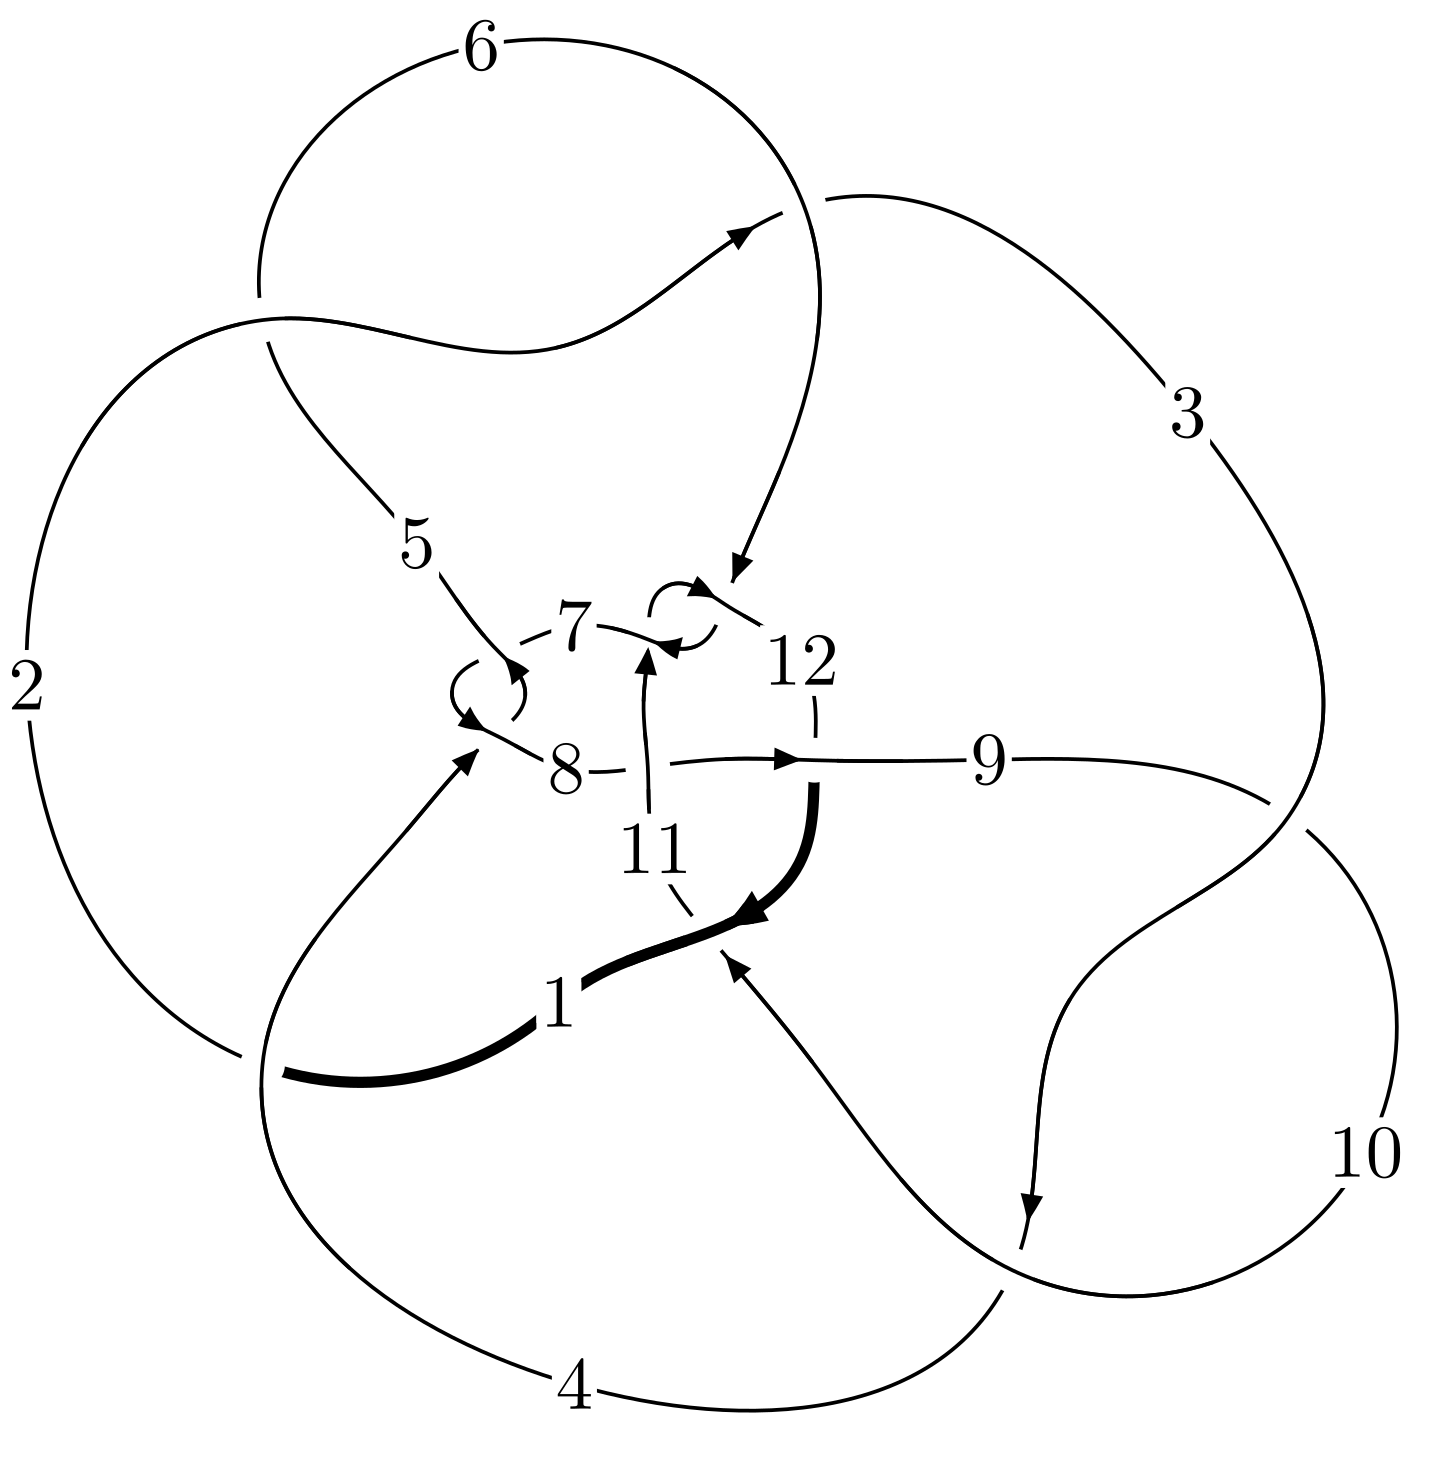
\includegraphics[width=112pt]{../../../GIT/diagram.site/Diagrams/png/1749_12a_0948.png}\\
\ \ \ A knot diagram\footnotemark}&
\allowdisplaybreaks
\textbf{Linearized knot diagam} \\
\cline{2-2}
 &
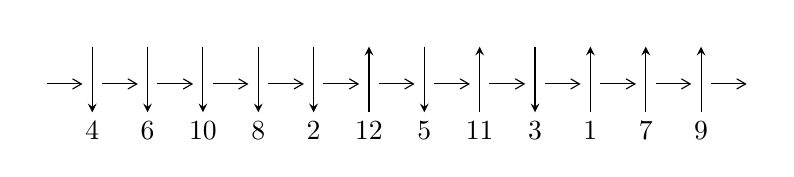
\begin{tikzpicture}[x=20pt, y=17pt]
	% nodes
	\node (C0) at (0, 0) {};
	\node (C1) at (1, 0) {};
	\node (C1U) at (1, +1) {};
	\node (C1D) at (1, -1) {4};

	\node (C2) at (2, 0) {};
	\node (C2U) at (2, +1) {};
	\node (C2D) at (2, -1) {6};

	\node (C3) at (3, 0) {};
	\node (C3U) at (3, +1) {};
	\node (C3D) at (3, -1) {10};

	\node (C4) at (4, 0) {};
	\node (C4U) at (4, +1) {};
	\node (C4D) at (4, -1) {8};

	\node (C5) at (5, 0) {};
	\node (C5U) at (5, +1) {};
	\node (C5D) at (5, -1) {2};

	\node (C6) at (6, 0) {};
	\node (C6U) at (6, +1) {};
	\node (C6D) at (6, -1) {12};

	\node (C7) at (7, 0) {};
	\node (C7U) at (7, +1) {};
	\node (C7D) at (7, -1) {5};

	\node (C8) at (8, 0) {};
	\node (C8U) at (8, +1) {};
	\node (C8D) at (8, -1) {11};

	\node (C9) at (9, 0) {};
	\node (C9U) at (9, +1) {};
	\node (C9D) at (9, -1) {3};

	\node (C10) at (10, 0) {};
	\node (C10U) at (10, +1) {};
	\node (C10D) at (10, -1) {1};

	\node (C11) at (11, 0) {};
	\node (C11U) at (11, +1) {};
	\node (C11D) at (11, -1) {7};

	\node (C12) at (12, 0) {};
	\node (C12U) at (12, +1) {};
	\node (C12D) at (12, -1) {9};
	\node (C13) at (13, 0) {};

	% arrows
	\draw[->,>={angle 60}]
	(C0) edge (C1) (C1) edge (C2) (C2) edge (C3) (C3) edge (C4) (C4) edge (C5) (C5) edge (C6) (C6) edge (C7) (C7) edge (C8) (C8) edge (C9) (C9) edge (C10) (C10) edge (C11) (C11) edge (C12) (C12) edge (C13) ;	\draw[->,>=stealth]
	(C1U) edge (C1D) (C2U) edge (C2D) (C3U) edge (C3D) (C4U) edge (C4D) (C5U) edge (C5D) (C6D) edge (C6U) (C7U) edge (C7D) (C8D) edge (C8U) (C9U) edge (C9D) (C10D) edge (C10U) (C11D) edge (C11U) (C12D) edge (C12U) ;
	\end{tikzpicture} \\
\hhline{~~} \\& 
\textbf{Solving Sequence} \\ \cline{2-2} 
 &
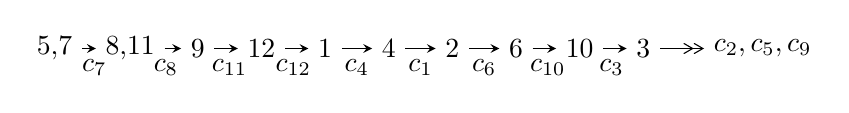
\begin{tikzpicture}[x=23pt, y=7pt]
	% node
	\node (A0) at (-1/8, 0) {5,7};
	\node (A1) at (17/16, 0) {8,11};
	\node (A2) at (17/8, 0) {9};
	\node (A3) at (25/8, 0) {12};
	\node (A4) at (33/8, 0) {1};
	\node (A5) at (41/8, 0) {4};
	\node (A6) at (49/8, 0) {2};
	\node (A7) at (57/8, 0) {6};
	\node (A8) at (65/8, 0) {10};
	\node (A9) at (73/8, 0) {3};
	\node (C1) at (1/2, -1) {$c_{7}$};
	\node (C2) at (13/8, -1) {$c_{8}$};
	\node (C3) at (21/8, -1) {$c_{11}$};
	\node (C4) at (29/8, -1) {$c_{12}$};
	\node (C5) at (37/8, -1) {$c_{4}$};
	\node (C6) at (45/8, -1) {$c_{1}$};
	\node (C7) at (53/8, -1) {$c_{6}$};
	\node (C8) at (61/8, -1) {$c_{10}$};
	\node (C9) at (69/8, -1) {$c_{3}$};
	\node (A10) at (11, 0) {$c_{2},c_{5},c_{9}$};

	% edge
	\draw[->,>=stealth]	
	(A0) edge (A1) (A1) edge (A2) (A2) edge (A3) (A3) edge (A4) (A4) edge (A5) (A5) edge (A6) (A6) edge (A7) (A7) edge (A8) (A8) edge (A9) ;
	\draw[->>,>={angle 60}]	
	(A9) edge (A10);
\end{tikzpicture} \\ 

\end{tabular} \\

\footnotetext{
The image of knot diagram is generated by the software ``\textbf{Draw programme}" developed by Andrew Bartholomew(\url{http://www.layer8.co.uk/maths/draw/index.htm\#Running-draw}), where we modified some parts for our purpose(\url{https://github.com/CATsTAILs/LinksPainter}).
}\phantom \\ \newline 
\centering \textbf{Ideals for irreducible components\footnotemark of $X_{\text{par}}$} 
 
\begin{align*}
I^u_{1}&=\langle 
4.82117\times10^{1053} u^{173}-4.17945\times10^{1054} u^{172}+\cdots+6.20593\times10^{1055} b-1.69443\times10^{1058},\\
\phantom{I^u_{1}}&\phantom{= \langle  }3.67137\times10^{1057} u^{173}-2.36071\times10^{1058} u^{172}+\cdots+9.41254\times10^{1059} a+2.24659\times10^{1060},\\
\phantom{I^u_{1}}&\phantom{= \langle  }u^{174}-8 u^{173}+\cdots-103455 u+15167\rangle \\
I^u_{2}&=\langle 
1.73012\times10^{65} u^{48}+9.41857\times10^{65} u^{47}+\cdots+3.09147\times10^{64} b-2.30301\times10^{64},\\
\phantom{I^u_{2}}&\phantom{= \langle  }-5.28502\times10^{65} u^{48}-2.32675\times10^{66} u^{47}+\cdots+3.09147\times10^{64} a+1.24633\times10^{66},\;u^{49}+5 u^{48}+\cdots+2 u+1\rangle \\
\\
\end{align*}
\raggedright * 2 irreducible components of $\dim_{\mathbb{C}}=0$, with total 223 representations.\\
\footnotetext{All coefficients of polynomials are rational numbers. But the coefficients are sometimes approximated in decimal forms when there is not enough margin.}
\newpage
\renewcommand{\arraystretch}{1}
\centering \section*{I. $I^u_{1}= \langle 4.82\times10^{1053} u^{173}-4.18\times10^{1054} u^{172}+\cdots+6.21\times10^{1055} b-1.69\times10^{1058},\;3.67\times10^{1057} u^{173}-2.36\times10^{1058} u^{172}+\cdots+9.41\times10^{1059} a+2.25\times10^{1060},\;u^{174}-8 u^{173}+\cdots-103455 u+15167 \rangle$}
\flushleft \textbf{(i) Arc colorings}\\
\begin{tabular}{m{7pt} m{180pt} m{7pt} m{180pt} }
\flushright $a_{5}=$&$\begin{pmatrix}0\\u\end{pmatrix}$ \\
\flushright $a_{7}=$&$\begin{pmatrix}1\\0\end{pmatrix}$ \\
\flushright $a_{8}=$&$\begin{pmatrix}1\\u^2\end{pmatrix}$ \\
\flushright $a_{11}=$&$\begin{pmatrix}-0.00390051 u^{173}+0.0250805 u^{172}+\cdots+71.5023 u-2.38681\\-0.00776864 u^{173}+0.0673460 u^{172}+\cdots-1844.78 u+273.033\end{pmatrix}$ \\
\flushright $a_{9}=$&$\begin{pmatrix}-0.000688694 u^{173}+0.0205837 u^{172}+\cdots-4667.87 u+756.663\\0.00312005 u^{173}-0.0195711 u^{172}+\cdots-923.636 u+179.023\end{pmatrix}$ \\
\flushright $a_{12}=$&$\begin{pmatrix}-0.0116691 u^{173}+0.0924265 u^{172}+\cdots-1773.28 u+270.646\\-0.00776864 u^{173}+0.0673460 u^{172}+\cdots-1844.78 u+273.033\end{pmatrix}$ \\
\flushright $a_{1}=$&$\begin{pmatrix}0.00293430 u^{173}-0.0302441 u^{172}+\cdots+653.871 u-107.847\\0.000613664 u^{173}-0.00576074 u^{172}+\cdots+666.345 u-89.8223\end{pmatrix}$ \\
\flushright $a_{4}=$&$\begin{pmatrix}u\\u^3+u\end{pmatrix}$ \\
\flushright $a_{2}=$&$\begin{pmatrix}0.000973190 u^{173}-0.0125045 u^{172}+\cdots+364.254 u-58.2403\\0.00127663 u^{173}-0.00949914 u^{172}+\cdots+618.636 u-71.3194\end{pmatrix}$ \\
\flushright $a_{6}=$&$\begin{pmatrix}-0.0114313 u^{173}+0.0803791 u^{172}+\cdots+950.078 u-226.104\\-0.00429712 u^{173}+0.0353554 u^{172}+\cdots-214.768 u+3.73542\end{pmatrix}$ \\
\flushright $a_{10}=$&$\begin{pmatrix}0.00643769 u^{173}-0.0520573 u^{172}+\cdots+832.298 u-55.2080\\0.00241189 u^{173}-0.0126908 u^{172}+\cdots-244.208 u+53.3806\end{pmatrix}$ \\
\flushright $a_{3}=$&$\begin{pmatrix}0.0172693 u^{173}-0.126967 u^{172}+\cdots-1235.18 u+312.981\\0.00834636 u^{173}-0.0675586 u^{172}+\cdots+1243.58 u-144.687\end{pmatrix}$\\&\end{tabular}
\flushleft \textbf{(ii) Obstruction class $= -1$}\\~\\
\flushleft \textbf{(iii) Cusp Shapes $= 0.0230806 u^{173}-0.156308 u^{172}+\cdots-3025.39 u+569.638$}\\~\\
\newpage\renewcommand{\arraystretch}{1}
\flushleft \textbf{(iv) u-Polynomials at the component}\newline \\
\begin{tabular}{m{50pt}|m{274pt}}
Crossings & \hspace{64pt}u-Polynomials at each crossing \\
\hline $$\begin{aligned}c_{1}\end{aligned}$$&$\begin{aligned}
&u^{174}-8 u^{173}+\cdots+43078027074 u-2742648543
\end{aligned}$\\
\hline $$\begin{aligned}c_{2},c_{5}\end{aligned}$$&$\begin{aligned}
&9(9 u^{174}+48 u^{173}+\cdots-1.82848\times10^{8} u-2.86544\times10^{7})
\end{aligned}$\\
\hline $$\begin{aligned}c_{3},c_{9}\end{aligned}$$&$\begin{aligned}
&u^{174}-3 u^{173}+\cdots+117419 u+88717
\end{aligned}$\\
\hline $$\begin{aligned}c_{4},c_{7}\end{aligned}$$&$\begin{aligned}
&u^{174}-8 u^{173}+\cdots-103455 u+15167
\end{aligned}$\\
\hline $$\begin{aligned}c_{6},c_{11}\end{aligned}$$&$\begin{aligned}
&9(9 u^{174}-6 u^{173}+\cdots+1495690 u-685471)
\end{aligned}$\\
\hline $$\begin{aligned}c_{8}\end{aligned}$$&$\begin{aligned}
&u^{174}+36 u^{173}+\cdots-108064167 u-3658113
\end{aligned}$\\
\hline $$\begin{aligned}c_{10}\end{aligned}$$&$\begin{aligned}
&81(81 u^{174}+2196 u^{173}+\cdots+9690823 u+854041)
\end{aligned}$\\
\hline $$\begin{aligned}c_{12}\end{aligned}$$&$\begin{aligned}
&u^{174}-4 u^{173}+\cdots-9297164295 u-155059353
\end{aligned}$\\
\hline
\end{tabular}\\~\\
\newpage\renewcommand{\arraystretch}{1}
\flushleft \textbf{(v) Riley Polynomials at the component}\newline \\
\begin{tabular}{m{50pt}|m{274pt}}
Crossings & \hspace{64pt}Riley Polynomials at each crossing \\
\hline $$\begin{aligned}c_{1}\end{aligned}$$&$\begin{aligned}
&y^{174}-36 y^{173}+\cdots-6.70\times10^{20} y+7.52\times10^{18}
\end{aligned}$\\
\hline $$\begin{aligned}c_{2},c_{5}\end{aligned}$$&$\begin{aligned}
&81\\
&\cdot(81 y^{174}-6552 y^{173}+\cdots+36023322668094366 y+821074238198449)
\end{aligned}$\\
\hline $$\begin{aligned}c_{3},c_{9}\end{aligned}$$&$\begin{aligned}
&y^{174}-135 y^{173}+\cdots-197112030361 y+7870706089
\end{aligned}$\\
\hline $$\begin{aligned}c_{4},c_{7}\end{aligned}$$&$\begin{aligned}
&y^{174}+82 y^{173}+\cdots+17293282263 y+230037889
\end{aligned}$\\
\hline $$\begin{aligned}c_{6},c_{11}\end{aligned}$$&$\begin{aligned}
&81\\
&\cdot(81 y^{174}+10134 y^{173}+\cdots+10182336694290 y+469870491841)
\end{aligned}$\\
\hline $$\begin{aligned}c_{8}\end{aligned}$$&$\begin{aligned}
&y^{174}-80 y^{173}+\cdots-218702911553847 y+13381790720769
\end{aligned}$\\
\hline $$\begin{aligned}c_{10}\end{aligned}$$&$\begin{aligned}
&6561\\
&\cdot(6561 y^{174}-435132 y^{173}+\cdots-22717612681479 y+729386029681)
\end{aligned}$\\
\hline $$\begin{aligned}c_{12}\end{aligned}$$&$\begin{aligned}
&y^{174}+52 y^{173}+\cdots-9052861972252739517 y+24043402952778609
\end{aligned}$\\
\hline
\end{tabular}\\~\\
\newpage\flushleft \textbf{(vi) Complex Volumes and Cusp Shapes}
$$\begin{array}{c|c|c}  
\text{Solutions to }I^u_{1}& \I (\text{vol} + \sqrt{-1}CS) & \text{Cusp shape}\\
 \hline 
\begin{aligned}
u &= \phantom{-}0.105788 + 0.992907 I \\
a &= -8.63885 + 2.18936 I \\
b &= \phantom{-}0.054244 + 1.013980 I\end{aligned}
 & -1.57777 - 0.35841 I & \phantom{-0.000000 } 0 \\ \hline\begin{aligned}
u &= \phantom{-}0.105788 - 0.992907 I \\
a &= -8.63885 - 2.18936 I \\
b &= \phantom{-}0.054244 - 1.013980 I\end{aligned}
 & -1.57777 + 0.35841 I & \phantom{-0.000000 } 0 \\ \hline\begin{aligned}
u &= \phantom{-}0.017165 + 1.001590 I \\
a &= \phantom{-}0.513932 + 0.985222 I \\
b &= -0.643237 - 0.876559 I\end{aligned}
 & -1.92649 + 4.95178 I & \phantom{-0.000000 } 0 \\ \hline\begin{aligned}
u &= \phantom{-}0.017165 - 1.001590 I \\
a &= \phantom{-}0.513932 - 0.985222 I \\
b &= -0.643237 + 0.876559 I\end{aligned}
 & -1.92649 - 4.95178 I & \phantom{-0.000000 } 0 \\ \hline\begin{aligned}
u &= -0.499108 + 0.863471 I \\
a &= \phantom{-}2.63700 + 0.62587 I \\
b &= -0.35250 - 2.71529 I\end{aligned}
 & -1.67953 + 2.03058 I & \phantom{-0.000000 } 0 \\ \hline\begin{aligned}
u &= -0.499108 - 0.863471 I \\
a &= \phantom{-}2.63700 - 0.62587 I \\
b &= -0.35250 + 2.71529 I\end{aligned}
 & -1.67953 - 2.03058 I & \phantom{-0.000000 } 0 \\ \hline\begin{aligned}
u &= \phantom{-}0.263655 + 0.974190 I \\
a &= \phantom{-}0.747181 - 0.626422 I \\
b &= -0.456440 + 0.019467 I\end{aligned}
 & -0.78721 - 2.39358 I & \phantom{-0.000000 } 0 \\ \hline\begin{aligned}
u &= \phantom{-}0.263655 - 0.974190 I \\
a &= \phantom{-}0.747181 + 0.626422 I \\
b &= -0.456440 - 0.019467 I\end{aligned}
 & -0.78721 + 2.39358 I & \phantom{-0.000000 } 0 \\ \hline\begin{aligned}
u &= \phantom{-}0.060232 + 0.986081 I \\
a &= -0.848099 - 0.131819 I \\
b &= \phantom{-}0.719978 + 0.392925 I\end{aligned}
 & \phantom{-}1.64504 + 1.44970 I & \phantom{-0.000000 } 0 \\ \hline\begin{aligned}
u &= \phantom{-}0.060232 - 0.986081 I \\
a &= -0.848099 + 0.131819 I \\
b &= \phantom{-}0.719978 - 0.392925 I\end{aligned}
 & \phantom{-}1.64504 - 1.44970 I & \phantom{-0.000000 } 0\\
 \hline 
 \end{array}$$\newpage$$\begin{array}{c|c|c}  
\text{Solutions to }I^u_{1}& \I (\text{vol} + \sqrt{-1}CS) & \text{Cusp shape}\\
 \hline 
\begin{aligned}
u &= -0.982738 + 0.245568 I \\
a &= -0.466688 + 0.751681 I \\
b &= \phantom{-}0.738446 + 0.146963 I\end{aligned}
 & -2.23933 - 2.59331 I & \phantom{-0.000000 } 0 \\ \hline\begin{aligned}
u &= -0.982738 - 0.245568 I \\
a &= -0.466688 - 0.751681 I \\
b &= \phantom{-}0.738446 - 0.146963 I\end{aligned}
 & -2.23933 + 2.59331 I & \phantom{-0.000000 } 0 \\ \hline\begin{aligned}
u &= \phantom{-}0.899970 + 0.474333 I \\
a &= -0.348297 - 0.228697 I \\
b &= -0.390896 - 1.211660 I\end{aligned}
 & -4.53629 + 3.07712 I & \phantom{-0.000000 } 0 \\ \hline\begin{aligned}
u &= \phantom{-}0.899970 - 0.474333 I \\
a &= -0.348297 + 0.228697 I \\
b &= -0.390896 + 1.211660 I\end{aligned}
 & -4.53629 - 3.07712 I & \phantom{-0.000000 } 0 \\ \hline\begin{aligned}
u &= -0.308477 + 0.973260 I \\
a &= -4.04787 + 0.47567 I \\
b &= \phantom{-}0.085823 + 1.000220 I\end{aligned}
 & -1.55044 + 1.07512 I & \phantom{-0.000000 } 0 \\ \hline\begin{aligned}
u &= -0.308477 - 0.973260 I \\
a &= -4.04787 - 0.47567 I \\
b &= \phantom{-}0.085823 - 1.000220 I\end{aligned}
 & -1.55044 - 1.07512 I & \phantom{-0.000000 } 0 \\ \hline\begin{aligned}
u &= \phantom{-}0.451931 + 0.862066 I \\
a &= -2.91381 + 0.21847 I \\
b &= \phantom{-}0.170072 - 1.326330 I\end{aligned}
 & -10.77750 - 6.33574 I & \phantom{-0.000000 } 0 \\ \hline\begin{aligned}
u &= \phantom{-}0.451931 - 0.862066 I \\
a &= -2.91381 - 0.21847 I \\
b &= \phantom{-}0.170072 + 1.326330 I\end{aligned}
 & -10.77750 + 6.33574 I & \phantom{-0.000000 } 0 \\ \hline\begin{aligned}
u &= -0.327654 + 0.978486 I \\
a &= -1.55074 + 0.46263 I \\
b &= \phantom{-}1.373920 - 0.100475 I\end{aligned}
 & \phantom{-}1.59680 + 3.06648 I & \phantom{-0.000000 } 0 \\ \hline\begin{aligned}
u &= -0.327654 - 0.978486 I \\
a &= -1.55074 - 0.46263 I \\
b &= \phantom{-}1.373920 + 0.100475 I\end{aligned}
 & \phantom{-}1.59680 - 3.06648 I & \phantom{-0.000000 } 0\\
 \hline 
 \end{array}$$\newpage$$\begin{array}{c|c|c}  
\text{Solutions to }I^u_{1}& \I (\text{vol} + \sqrt{-1}CS) & \text{Cusp shape}\\
 \hline 
\begin{aligned}
u &= \phantom{-}0.816236 + 0.518820 I \\
a &= -0.049880 + 0.592643 I \\
b &= -0.260211 + 1.308340 I\end{aligned}
 & -7.48812 - 6.13354 I & \phantom{-0.000000 } 0 \\ \hline\begin{aligned}
u &= \phantom{-}0.816236 - 0.518820 I \\
a &= -0.049880 - 0.592643 I \\
b &= -0.260211 - 1.308340 I\end{aligned}
 & -7.48812 + 6.13354 I & \phantom{-0.000000 } 0 \\ \hline\begin{aligned}
u &= \phantom{-}0.511228 + 0.814965 I \\
a &= -0.314456 - 0.613076 I \\
b &= -0.17044 - 1.55691 I\end{aligned}
 & -10.90080 + 2.39166 I & \phantom{-0.000000 } 0 \\ \hline\begin{aligned}
u &= \phantom{-}0.511228 - 0.814965 I \\
a &= -0.314456 + 0.613076 I \\
b &= -0.17044 + 1.55691 I\end{aligned}
 & -10.90080 - 2.39166 I & \phantom{-0.000000 } 0 \\ \hline\begin{aligned}
u &= \phantom{-}0.413407 + 0.957407 I \\
a &= \phantom{-}0.218950 - 0.495465 I \\
b &= \phantom{-}0.29409 + 1.80147 I\end{aligned}
 & -10.06320 - 6.70670 I & \phantom{-0.000000 } 0 \\ \hline\begin{aligned}
u &= \phantom{-}0.413407 - 0.957407 I \\
a &= \phantom{-}0.218950 + 0.495465 I \\
b &= \phantom{-}0.29409 - 1.80147 I\end{aligned}
 & -10.06320 + 6.70670 I & \phantom{-0.000000 } 0 \\ \hline\begin{aligned}
u &= -0.955084 + 0.055699 I \\
a &= -0.323674 - 0.044907 I \\
b &= \phantom{-}0.256490 - 1.100480 I\end{aligned}
 & -2.23201 - 3.29265 I & \phantom{-0.000000 } 0 \\ \hline\begin{aligned}
u &= -0.955084 - 0.055699 I \\
a &= -0.323674 + 0.044907 I \\
b &= \phantom{-}0.256490 + 1.100480 I\end{aligned}
 & -2.23201 + 3.29265 I & \phantom{-0.000000 } 0 \\ \hline\begin{aligned}
u &= \phantom{-}0.775120 + 0.559710 I \\
a &= \phantom{-}0.462315 + 0.172632 I \\
b &= \phantom{-}0.59221 + 1.40373 I\end{aligned}
 & -7.05184 + 5.89114 I & \phantom{-0.000000 } 0 \\ \hline\begin{aligned}
u &= \phantom{-}0.775120 - 0.559710 I \\
a &= \phantom{-}0.462315 - 0.172632 I \\
b &= \phantom{-}0.59221 - 1.40373 I\end{aligned}
 & -7.05184 - 5.89114 I & \phantom{-0.000000 } 0\\
 \hline 
 \end{array}$$\newpage$$\begin{array}{c|c|c}  
\text{Solutions to }I^u_{1}& \I (\text{vol} + \sqrt{-1}CS) & \text{Cusp shape}\\
 \hline 
\begin{aligned}
u &= \phantom{-}0.580676 + 0.881375 I \\
a &= \phantom{-}0.124712 + 0.086717 I \\
b &= -0.316735 - 1.354540 I\end{aligned}
 & -5.05541 - 3.45080 I & \phantom{-0.000000 } 0 \\ \hline\begin{aligned}
u &= \phantom{-}0.580676 - 0.881375 I \\
a &= \phantom{-}0.124712 - 0.086717 I \\
b &= -0.316735 + 1.354540 I\end{aligned}
 & -5.05541 + 3.45080 I & \phantom{-0.000000 } 0 \\ \hline\begin{aligned}
u &= -0.925467 + 0.165358 I \\
a &= \phantom{-}0.212828 - 1.017190 I \\
b &= -0.962519 - 0.132593 I\end{aligned}
 & -6.30291 - 8.32375 I & \phantom{-0.000000 } 0 \\ \hline\begin{aligned}
u &= -0.925467 - 0.165358 I \\
a &= \phantom{-}0.212828 + 1.017190 I \\
b &= -0.962519 + 0.132593 I\end{aligned}
 & -6.30291 + 8.32375 I & \phantom{-0.000000 } 0 \\ \hline\begin{aligned}
u &= \phantom{-}0.598860 + 0.721099 I \\
a &= -2.31654 - 0.04429 I \\
b &= \phantom{-}0.490731 - 1.112850 I\end{aligned}
 & -5.53054 - 1.20802 I & \phantom{-0.000000 } 0 \\ \hline\begin{aligned}
u &= \phantom{-}0.598860 - 0.721099 I \\
a &= -2.31654 + 0.04429 I \\
b &= \phantom{-}0.490731 + 1.112850 I\end{aligned}
 & -5.53054 + 1.20802 I & \phantom{-0.000000 } 0 \\ \hline\begin{aligned}
u &= -1.043250 + 0.217868 I \\
a &= \phantom{-}0.208576 - 0.431210 I \\
b &= -0.670560 + 0.335177 I\end{aligned}
 & -6.81979 + 2.60677 I & \phantom{-0.000000 } 0 \\ \hline\begin{aligned}
u &= -1.043250 - 0.217868 I \\
a &= \phantom{-}0.208576 + 0.431210 I \\
b &= -0.670560 - 0.335177 I\end{aligned}
 & -6.81979 - 2.60677 I & \phantom{-0.000000 } 0 \\ \hline\begin{aligned}
u &= -0.123285 + 1.067010 I \\
a &= \phantom{-}1.68532 - 0.19184 I \\
b &= -0.546914 - 0.708360 I\end{aligned}
 & \phantom{-}4.45474 + 0.18317 I & \phantom{-0.000000 } 0 \\ \hline\begin{aligned}
u &= -0.123285 - 1.067010 I \\
a &= \phantom{-}1.68532 + 0.19184 I \\
b &= -0.546914 + 0.708360 I\end{aligned}
 & \phantom{-}4.45474 - 0.18317 I & \phantom{-0.000000 } 0\\
 \hline 
 \end{array}$$\newpage$$\begin{array}{c|c|c}  
\text{Solutions to }I^u_{1}& \I (\text{vol} + \sqrt{-1}CS) & \text{Cusp shape}\\
 \hline 
\begin{aligned}
u &= -0.633347 + 0.674496 I \\
a &= \phantom{-}0.91686 - 1.35419 I \\
b &= -0.735016 - 0.367384 I\end{aligned}
 & -0.91675 + 1.10715 I & \phantom{-0.000000 } 0 \\ \hline\begin{aligned}
u &= -0.633347 - 0.674496 I \\
a &= \phantom{-}0.91686 + 1.35419 I \\
b &= -0.735016 + 0.367384 I\end{aligned}
 & -0.91675 - 1.10715 I & \phantom{-0.000000 } 0 \\ \hline\begin{aligned}
u &= \phantom{-}0.060216 + 1.074030 I \\
a &= -1.48380 - 0.47596 I \\
b &= \phantom{-}0.877280 + 0.288988 I\end{aligned}
 & \phantom{-}3.09545 + 3.19700 I & \phantom{-0.000000 } 0 \\ \hline\begin{aligned}
u &= \phantom{-}0.060216 - 1.074030 I \\
a &= -1.48380 + 0.47596 I \\
b &= \phantom{-}0.877280 - 0.288988 I\end{aligned}
 & \phantom{-}3.09545 - 3.19700 I & \phantom{-0.000000 } 0 \\ \hline\begin{aligned}
u &= -0.281831 + 0.874245 I \\
a &= \phantom{-}1.94112 - 0.86508 I \\
b &= -1.42405 + 0.33650 I\end{aligned}
 & \phantom{-}1.150790 - 0.546322 I & \phantom{-0.000000 } 0 \\ \hline\begin{aligned}
u &= -0.281831 - 0.874245 I \\
a &= \phantom{-}1.94112 + 0.86508 I \\
b &= -1.42405 - 0.33650 I\end{aligned}
 & \phantom{-}1.150790 + 0.546322 I & \phantom{-0.000000 } 0 \\ \hline\begin{aligned}
u &= \phantom{-}0.363643 + 1.030730 I \\
a &= \phantom{-}1.43406 + 0.54770 I \\
b &= -0.797668 - 0.411576 I\end{aligned}
 & \phantom{-}3.31463 - 3.43074 I & \phantom{-0.000000 } 0 \\ \hline\begin{aligned}
u &= \phantom{-}0.363643 - 1.030730 I \\
a &= \phantom{-}1.43406 - 0.54770 I \\
b &= -0.797668 + 0.411576 I\end{aligned}
 & \phantom{-}3.31463 + 3.43074 I & \phantom{-0.000000 } 0 \\ \hline\begin{aligned}
u &= -0.868376 + 0.248762 I \\
a &= \phantom{-}0.321564 + 0.289191 I \\
b &= -0.317728 + 1.303600 I\end{aligned}
 & -6.06536 - 8.12155 I & \phantom{-0.000000 } 0 \\ \hline\begin{aligned}
u &= -0.868376 - 0.248762 I \\
a &= \phantom{-}0.321564 - 0.289191 I \\
b &= -0.317728 - 1.303600 I\end{aligned}
 & -6.06536 + 8.12155 I & \phantom{-0.000000 } 0\\
 \hline 
 \end{array}$$\newpage$$\begin{array}{c|c|c}  
\text{Solutions to }I^u_{1}& \I (\text{vol} + \sqrt{-1}CS) & \text{Cusp shape}\\
 \hline 
\begin{aligned}
u &= \phantom{-}0.023259 + 0.900920 I \\
a &= \phantom{-}2.11030 + 0.43584 I \\
b &= -0.387990 - 0.304064 I\end{aligned}
 & \phantom{-}4.12487 + 0.03193 I & \phantom{-0.000000 } 0 \\ \hline\begin{aligned}
u &= \phantom{-}0.023259 - 0.900920 I \\
a &= \phantom{-}2.11030 - 0.43584 I \\
b &= -0.387990 + 0.304064 I\end{aligned}
 & \phantom{-}4.12487 - 0.03193 I & \phantom{-0.000000 } 0 \\ \hline\begin{aligned}
u &= \phantom{-}0.457284 + 1.002900 I \\
a &= -1.48423 - 0.65641 I \\
b &= \phantom{-}0.853354 + 0.096959 I\end{aligned}
 & \phantom{-}0.41605 - 8.37907 I & \phantom{-0.000000 } 0 \\ \hline\begin{aligned}
u &= \phantom{-}0.457284 - 1.002900 I \\
a &= -1.48423 + 0.65641 I \\
b &= \phantom{-}0.853354 - 0.096959 I\end{aligned}
 & \phantom{-}0.41605 + 8.37907 I & \phantom{-0.000000 } 0 \\ \hline\begin{aligned}
u &= -0.585126 + 0.664641 I \\
a &= -0.633629 - 0.213282 I \\
b &= -0.209969 + 1.210890 I\end{aligned}
 & -1.60446 + 1.50746 I & \phantom{-0.000000 } 0 \\ \hline\begin{aligned}
u &= -0.585126 - 0.664641 I \\
a &= -0.633629 + 0.213282 I \\
b &= -0.209969 - 1.210890 I\end{aligned}
 & -1.60446 - 1.50746 I & \phantom{-0.000000 } 0 \\ \hline\begin{aligned}
u &= -1.026190 + 0.442963 I \\
a &= \phantom{-}0.275739 + 0.036861 I \\
b &= \phantom{-}0.332904 + 0.700789 I\end{aligned}
 & -5.42577 + 2.00818 I & \phantom{-0.000000 } 0 \\ \hline\begin{aligned}
u &= -1.026190 - 0.442963 I \\
a &= \phantom{-}0.275739 - 0.036861 I \\
b &= \phantom{-}0.332904 - 0.700789 I\end{aligned}
 & -5.42577 - 2.00818 I & \phantom{-0.000000 } 0 \\ \hline\begin{aligned}
u &= \phantom{-}0.634590 + 0.920462 I \\
a &= -1.48155 + 0.01846 I \\
b &= \phantom{-}0.061580 - 0.909578 I\end{aligned}
 & -4.25232 - 0.64086 I & \phantom{-0.000000 } 0 \\ \hline\begin{aligned}
u &= \phantom{-}0.634590 - 0.920462 I \\
a &= -1.48155 - 0.01846 I \\
b &= \phantom{-}0.061580 + 0.909578 I\end{aligned}
 & -4.25232 + 0.64086 I & \phantom{-0.000000 } 0\\
 \hline 
 \end{array}$$\newpage$$\begin{array}{c|c|c}  
\text{Solutions to }I^u_{1}& \I (\text{vol} + \sqrt{-1}CS) & \text{Cusp shape}\\
 \hline 
\begin{aligned}
u &= -0.755027 + 0.454788 I \\
a &= -0.053718 + 0.579396 I \\
b &= \phantom{-}0.201867 - 1.087000 I\end{aligned}
 & -5.29516 - 0.53701 I & \phantom{-0.000000 } 0 \\ \hline\begin{aligned}
u &= -0.755027 - 0.454788 I \\
a &= -0.053718 - 0.579396 I \\
b &= \phantom{-}0.201867 + 1.087000 I\end{aligned}
 & -5.29516 + 0.53701 I & \phantom{-0.000000 } 0 \\ \hline\begin{aligned}
u &= \phantom{-}0.540023 + 0.694861 I \\
a &= -0.153158 - 0.361356 I \\
b &= \phantom{-}0.055703 - 1.333580 I\end{aligned}
 & -4.98380 - 4.10822 I & \phantom{-0.000000 } 0 \\ \hline\begin{aligned}
u &= \phantom{-}0.540023 - 0.694861 I \\
a &= -0.153158 + 0.361356 I \\
b &= \phantom{-}0.055703 + 1.333580 I\end{aligned}
 & -4.98380 + 4.10822 I & \phantom{-0.000000 } 0 \\ \hline\begin{aligned}
u &= -1.101610 + 0.222702 I \\
a &= -0.047393 - 0.143697 I \\
b &= -0.193424 - 1.110190 I\end{aligned}
 & -5.87532 + 0.93957 I & \phantom{-0.000000 } 0 \\ \hline\begin{aligned}
u &= -1.101610 - 0.222702 I \\
a &= -0.047393 + 0.143697 I \\
b &= -0.193424 + 1.110190 I\end{aligned}
 & -5.87532 - 0.93957 I & \phantom{-0.000000 } 0 \\ \hline\begin{aligned}
u &= \phantom{-}0.093657 + 1.135620 I \\
a &= -1.409940 + 0.061582 I \\
b &= \phantom{-}1.216810 + 0.353798 I\end{aligned}
 & \phantom{-}1.74865 + 0.27878 I & \phantom{-0.000000 } 0 \\ \hline\begin{aligned}
u &= \phantom{-}0.093657 - 1.135620 I \\
a &= -1.409940 - 0.061582 I \\
b &= \phantom{-}1.216810 - 0.353798 I\end{aligned}
 & \phantom{-}1.74865 - 0.27878 I & \phantom{-0.000000 } 0 \\ \hline\begin{aligned}
u &= \phantom{-}0.151202 + 0.840096 I \\
a &= -1.83080 - 0.45938 I \\
b &= \phantom{-}0.263553 + 0.727900 I\end{aligned}
 & -1.45687 + 0.18954 I & \phantom{-0.000000 } 0 \\ \hline\begin{aligned}
u &= \phantom{-}0.151202 - 0.840096 I \\
a &= -1.83080 + 0.45938 I \\
b &= \phantom{-}0.263553 - 0.727900 I\end{aligned}
 & -1.45687 - 0.18954 I & \phantom{-0.000000 } 0\\
 \hline 
 \end{array}$$\newpage$$\begin{array}{c|c|c}  
\text{Solutions to }I^u_{1}& \I (\text{vol} + \sqrt{-1}CS) & \text{Cusp shape}\\
 \hline 
\begin{aligned}
u &= \phantom{-}0.431718 + 0.731263 I \\
a &= \phantom{-}2.69232 - 0.83150 I \\
b &= -0.44316 + 1.42863 I\end{aligned}
 & -10.80750 + 3.15916 I & \phantom{-0.000000 } 0 \\ \hline\begin{aligned}
u &= \phantom{-}0.431718 - 0.731263 I \\
a &= \phantom{-}2.69232 + 0.83150 I \\
b &= -0.44316 - 1.42863 I\end{aligned}
 & -10.80750 - 3.15916 I & \phantom{-0.000000 } 0 \\ \hline\begin{aligned}
u &= \phantom{-}0.002875 + 1.153440 I \\
a &= \phantom{-}1.51108 + 0.02918 I \\
b &= -1.28401 - 0.78539 I\end{aligned}
 & \phantom{-}1.15212 + 1.20462 I & \phantom{-0.000000 } 0 \\ \hline\begin{aligned}
u &= \phantom{-}0.002875 - 1.153440 I \\
a &= \phantom{-}1.51108 - 0.02918 I \\
b &= -1.28401 + 0.78539 I\end{aligned}
 & \phantom{-}1.15212 - 1.20462 I & \phantom{-0.000000 } 0 \\ \hline\begin{aligned}
u &= \phantom{-}0.454876 + 1.096400 I \\
a &= \phantom{-}1.83521 - 0.50281 I \\
b &= -0.61371 + 1.32945 I\end{aligned}
 & -2.41790 - 6.36783 I & \phantom{-0.000000 } 0 \\ \hline\begin{aligned}
u &= \phantom{-}0.454876 - 1.096400 I \\
a &= \phantom{-}1.83521 + 0.50281 I \\
b &= -0.61371 - 1.32945 I\end{aligned}
 & -2.41790 + 6.36783 I & \phantom{-0.000000 } 0 \\ \hline\begin{aligned}
u &= -0.468627 + 1.111020 I \\
a &= -0.792736 + 0.082852 I \\
b &= \phantom{-}0.818556 - 0.067626 I\end{aligned}
 & \phantom{-}0.84886 + 3.29889 I & \phantom{-0.000000 } 0 \\ \hline\begin{aligned}
u &= -0.468627 - 1.111020 I \\
a &= -0.792736 - 0.082852 I \\
b &= \phantom{-}0.818556 + 0.067626 I\end{aligned}
 & \phantom{-}0.84886 - 3.29889 I & \phantom{-0.000000 } 0 \\ \hline\begin{aligned}
u &= -0.574851 + 1.061100 I \\
a &= -1.297480 + 0.074808 I \\
b &= \phantom{-}0.573140 + 1.057110 I\end{aligned}
 & -0.12987 + 3.39369 I & \phantom{-0.000000 } 0 \\ \hline\begin{aligned}
u &= -0.574851 - 1.061100 I \\
a &= -1.297480 - 0.074808 I \\
b &= \phantom{-}0.573140 - 1.057110 I\end{aligned}
 & -0.12987 - 3.39369 I & \phantom{-0.000000 } 0\\
 \hline 
 \end{array}$$\newpage$$\begin{array}{c|c|c}  
\text{Solutions to }I^u_{1}& \I (\text{vol} + \sqrt{-1}CS) & \text{Cusp shape}\\
 \hline 
\begin{aligned}
u &= \phantom{-}0.969955 + 0.722466 I \\
a &= \phantom{-}0.495633 + 0.955340 I \\
b &= -0.047454 + 0.888667 I\end{aligned}
 & -0.36490 - 2.68762 I & \phantom{-0.000000 } 0 \\ \hline\begin{aligned}
u &= \phantom{-}0.969955 - 0.722466 I \\
a &= \phantom{-}0.495633 - 0.955340 I \\
b &= -0.047454 - 0.888667 I\end{aligned}
 & -0.36490 + 2.68762 I & \phantom{-0.000000 } 0 \\ \hline\begin{aligned}
u &= \phantom{-}0.453692 + 1.128250 I \\
a &= -1.18972 - 1.10940 I \\
b &= \phantom{-}0.280444 - 1.251060 I\end{aligned}
 & -5.47780 - 10.52790 I & \phantom{-0.000000 } 0 \\ \hline\begin{aligned}
u &= \phantom{-}0.453692 - 1.128250 I \\
a &= -1.18972 + 1.10940 I \\
b &= \phantom{-}0.280444 + 1.251060 I\end{aligned}
 & -5.47780 + 10.52790 I & \phantom{-0.000000 } 0 \\ \hline\begin{aligned}
u &= \phantom{-}0.622518 + 1.048770 I \\
a &= -0.812514 - 0.536519 I \\
b &= \phantom{-}0.082243 - 0.898246 I\end{aligned}
 & -0.44233 + 2.84121 I & \phantom{-0.000000 } 0 \\ \hline\begin{aligned}
u &= \phantom{-}0.622518 - 1.048770 I \\
a &= -0.812514 + 0.536519 I \\
b &= \phantom{-}0.082243 + 0.898246 I\end{aligned}
 & -0.44233 - 2.84121 I & \phantom{-0.000000 } 0 \\ \hline\begin{aligned}
u &= \phantom{-}0.583693 + 0.509936 I \\
a &= \phantom{-}2.86879 + 0.82366 I \\
b &= -0.721821 + 1.041950 I\end{aligned}
 & -8.46291 - 7.57961 I & \phantom{-0.000000 } 0 \\ \hline\begin{aligned}
u &= \phantom{-}0.583693 - 0.509936 I \\
a &= \phantom{-}2.86879 - 0.82366 I \\
b &= -0.721821 - 1.041950 I\end{aligned}
 & -8.46291 + 7.57961 I & \phantom{-0.000000 } 0 \\ \hline\begin{aligned}
u &= \phantom{-}0.745171 + 0.972980 I \\
a &= \phantom{-}1.274660 + 0.084117 I \\
b &= \phantom{-}0.207915 + 1.005180 I\end{aligned}
 & -6.24656 + 0.29952 I & \phantom{-0.000000 } 0 \\ \hline\begin{aligned}
u &= \phantom{-}0.745171 - 0.972980 I \\
a &= \phantom{-}1.274660 - 0.084117 I \\
b &= \phantom{-}0.207915 - 1.005180 I\end{aligned}
 & -6.24656 - 0.29952 I & \phantom{-0.000000 } 0\\
 \hline 
 \end{array}$$\newpage$$\begin{array}{c|c|c}  
\text{Solutions to }I^u_{1}& \I (\text{vol} + \sqrt{-1}CS) & \text{Cusp shape}\\
 \hline 
\begin{aligned}
u &= \phantom{-}0.798382 + 0.935782 I \\
a &= -1.036420 - 0.734833 I \\
b &= \phantom{-}0.361463 - 0.891330 I\end{aligned}
 & -0.99518 - 8.59993 I & \phantom{-0.000000 } 0 \\ \hline\begin{aligned}
u &= \phantom{-}0.798382 - 0.935782 I \\
a &= -1.036420 + 0.734833 I \\
b &= \phantom{-}0.361463 + 0.891330 I\end{aligned}
 & -0.99518 + 8.59993 I & \phantom{-0.000000 } 0 \\ \hline\begin{aligned}
u &= \phantom{-}0.637912 + 1.056310 I \\
a &= \phantom{-}1.80510 + 0.26388 I \\
b &= -0.75884 + 1.48150 I\end{aligned}
 & -5.54132 - 11.24360 I & \phantom{-0.000000 } 0 \\ \hline\begin{aligned}
u &= \phantom{-}0.637912 - 1.056310 I \\
a &= \phantom{-}1.80510 - 0.26388 I \\
b &= -0.75884 - 1.48150 I\end{aligned}
 & -5.54132 + 11.24360 I & \phantom{-0.000000 } 0 \\ \hline\begin{aligned}
u &= \phantom{-}0.631103 + 1.071510 I \\
a &= -0.412700 - 0.325772 I \\
b &= \phantom{-}0.64430 + 1.32236 I\end{aligned}
 & -6.77712 + 2.68736 I & \phantom{-0.000000 } 0 \\ \hline\begin{aligned}
u &= \phantom{-}0.631103 - 1.071510 I \\
a &= -0.412700 + 0.325772 I \\
b &= \phantom{-}0.64430 - 1.32236 I\end{aligned}
 & -6.77712 - 2.68736 I & \phantom{-0.000000 } 0 \\ \hline\begin{aligned}
u &= \phantom{-}0.590990 + 1.135850 I \\
a &= \phantom{-}1.147040 + 0.552687 I \\
b &= -0.206241 + 1.028440 I\end{aligned}
 & \phantom{-}1.47487 - 3.22310 I & \phantom{-0.000000 } 0 \\ \hline\begin{aligned}
u &= \phantom{-}0.590990 - 1.135850 I \\
a &= \phantom{-}1.147040 - 0.552687 I \\
b &= -0.206241 - 1.028440 I\end{aligned}
 & \phantom{-}1.47487 + 3.22310 I & \phantom{-0.000000 } 0 \\ \hline\begin{aligned}
u &= -0.722405 + 1.066110 I \\
a &= -0.708294 + 0.039478 I \\
b &= -0.020913 + 0.233589 I\end{aligned}
 & -3.58239 + 4.26656 I & \phantom{-0.000000 } 0 \\ \hline\begin{aligned}
u &= -0.722405 - 1.066110 I \\
a &= -0.708294 - 0.039478 I \\
b &= -0.020913 - 0.233589 I\end{aligned}
 & -3.58239 - 4.26656 I & \phantom{-0.000000 } 0\\
 \hline 
 \end{array}$$\newpage$$\begin{array}{c|c|c}  
\text{Solutions to }I^u_{1}& \I (\text{vol} + \sqrt{-1}CS) & \text{Cusp shape}\\
 \hline 
\begin{aligned}
u &= \phantom{-}0.665368 + 1.127100 I \\
a &= -1.41992 - 0.14541 I \\
b &= \phantom{-}0.61247 - 1.30407 I\end{aligned}
 & -2.55376 - 8.83647 I & \phantom{-0.000000 } 0 \\ \hline\begin{aligned}
u &= \phantom{-}0.665368 - 1.127100 I \\
a &= -1.41992 + 0.14541 I \\
b &= \phantom{-}0.61247 + 1.30407 I\end{aligned}
 & -2.55376 + 8.83647 I & \phantom{-0.000000 } 0 \\ \hline\begin{aligned}
u &= \phantom{-}0.102007 + 0.682962 I \\
a &= -1.76914 - 0.25695 I \\
b &= \phantom{-}0.44987 - 1.41245 I\end{aligned}
 & -4.14146 - 5.79026 I & \phantom{-0.000000 } 0 \\ \hline\begin{aligned}
u &= \phantom{-}0.102007 - 0.682962 I \\
a &= -1.76914 + 0.25695 I \\
b &= \phantom{-}0.44987 + 1.41245 I\end{aligned}
 & -4.14146 + 5.79026 I & \phantom{-0.000000 } 0 \\ \hline\begin{aligned}
u &= \phantom{-}1.238880 + 0.444512 I \\
a &= \phantom{-}0.090410 - 0.181053 I \\
b &= -0.564035 - 1.282780 I\end{aligned}
 & -9.8173 + 13.8772 I & \phantom{-0.000000 } 0 \\ \hline\begin{aligned}
u &= \phantom{-}1.238880 - 0.444512 I \\
a &= \phantom{-}0.090410 + 0.181053 I \\
b &= -0.564035 + 1.282780 I\end{aligned}
 & -9.8173 - 13.8772 I & \phantom{-0.000000 } 0 \\ \hline\begin{aligned}
u &= -0.590781 + 1.176220 I \\
a &= -1.81293 - 0.15426 I \\
b &= \phantom{-}0.506160 + 1.298340 I\end{aligned}
 & -3.35110 + 13.46760 I & \phantom{-0.000000 } 0 \\ \hline\begin{aligned}
u &= -0.590781 - 1.176220 I \\
a &= -1.81293 + 0.15426 I \\
b &= \phantom{-}0.506160 - 1.298340 I\end{aligned}
 & -3.35110 - 13.46760 I & \phantom{-0.000000 } 0 \\ \hline\begin{aligned}
u &= -0.534335 + 0.421295 I \\
a &= -0.678665 + 0.247161 I \\
b &= -0.023937 + 1.138570 I\end{aligned}
 & -1.63591 + 1.46544 I & \phantom{-0.000000 } 0 \\ \hline\begin{aligned}
u &= -0.534335 - 0.421295 I \\
a &= -0.678665 - 0.247161 I \\
b &= -0.023937 - 1.138570 I\end{aligned}
 & -1.63591 - 1.46544 I & \phantom{-0.000000 } 0\\
 \hline 
 \end{array}$$\newpage$$\begin{array}{c|c|c}  
\text{Solutions to }I^u_{1}& \I (\text{vol} + \sqrt{-1}CS) & \text{Cusp shape}\\
 \hline 
\begin{aligned}
u &= \phantom{-}0.498382 + 1.231610 I \\
a &= -1.40992 + 0.45423 I \\
b &= \phantom{-}0.62903 - 1.46229 I\end{aligned}
 & -3.03939 - 10.04370 I & \phantom{-0.000000 } 0 \\ \hline\begin{aligned}
u &= \phantom{-}0.498382 - 1.231610 I \\
a &= -1.40992 - 0.45423 I \\
b &= \phantom{-}0.62903 + 1.46229 I\end{aligned}
 & -3.03939 + 10.04370 I & \phantom{-0.000000 } 0 \\ \hline\begin{aligned}
u &= -0.646745 + 1.161720 I \\
a &= \phantom{-}1.005690 + 0.131636 I \\
b &= -0.530877 - 0.940813 I\end{aligned}
 & -3.09487 + 5.84029 I & \phantom{-0.000000 } 0 \\ \hline\begin{aligned}
u &= -0.646745 - 1.161720 I \\
a &= \phantom{-}1.005690 - 0.131636 I \\
b &= -0.530877 + 0.940813 I\end{aligned}
 & -3.09487 - 5.84029 I & \phantom{-0.000000 } 0 \\ \hline\begin{aligned}
u &= -0.524563 + 1.224790 I \\
a &= \phantom{-}1.64082 + 0.37202 I \\
b &= -0.543452 - 1.076860 I\end{aligned}
 & \phantom{-}1.25183 + 8.42208 I & \phantom{-0.000000 } 0 \\ \hline\begin{aligned}
u &= -0.524563 - 1.224790 I \\
a &= \phantom{-}1.64082 - 0.37202 I \\
b &= -0.543452 + 1.076860 I\end{aligned}
 & \phantom{-}1.25183 - 8.42208 I & \phantom{-0.000000 } 0 \\ \hline\begin{aligned}
u &= -0.608253 + 1.187600 I \\
a &= \phantom{-}1.046230 - 0.532919 I \\
b &= -1.110490 + 0.208651 I\end{aligned}
 & \phantom{-}0.56642 + 8.23567 I & \phantom{-0.000000 } 0 \\ \hline\begin{aligned}
u &= -0.608253 - 1.187600 I \\
a &= \phantom{-}1.046230 + 0.532919 I \\
b &= -1.110490 - 0.208651 I\end{aligned}
 & \phantom{-}0.56642 - 8.23567 I & \phantom{-0.000000 } 0 \\ \hline\begin{aligned}
u &= -0.579509 + 1.211110 I \\
a &= -1.152770 + 0.575913 I \\
b &= \phantom{-}1.382860 - 0.185529 I\end{aligned}
 & -3.22713 + 13.72270 I & \phantom{-0.000000 } 0 \\ \hline\begin{aligned}
u &= -0.579509 - 1.211110 I \\
a &= -1.152770 - 0.575913 I \\
b &= \phantom{-}1.382860 + 0.185529 I\end{aligned}
 & -3.22713 - 13.72270 I & \phantom{-0.000000 } 0\\
 \hline 
 \end{array}$$\newpage$$\begin{array}{c|c|c}  
\text{Solutions to }I^u_{1}& \I (\text{vol} + \sqrt{-1}CS) & \text{Cusp shape}\\
 \hline 
\begin{aligned}
u &= -0.130120 + 1.336890 I \\
a &= \phantom{-}0.993158 + 0.699794 I \\
b &= -0.453590 - 0.879843 I\end{aligned}
 & \phantom{-}3.90624 + 3.94646 I & \phantom{-0.000000 } 0 \\ \hline\begin{aligned}
u &= -0.130120 - 1.336890 I \\
a &= \phantom{-}0.993158 - 0.699794 I \\
b &= -0.453590 + 0.879843 I\end{aligned}
 & \phantom{-}3.90624 - 3.94646 I & \phantom{-0.000000 } 0 \\ \hline\begin{aligned}
u &= -0.292621 + 1.314260 I \\
a &= \phantom{-}0.258085 - 0.662559 I \\
b &= -0.132899 + 0.683008 I\end{aligned}
 & \phantom{-}2.69005 + 1.40993 I & \phantom{-0.000000 } 0 \\ \hline\begin{aligned}
u &= -0.292621 - 1.314260 I \\
a &= \phantom{-}0.258085 + 0.662559 I \\
b &= -0.132899 - 0.683008 I\end{aligned}
 & \phantom{-}2.69005 - 1.40993 I & \phantom{-0.000000 } 0 \\ \hline\begin{aligned}
u &= \phantom{-}1.248410 + 0.516227 I \\
a &= -0.196618 + 0.227169 I \\
b &= \phantom{-}0.492989 + 1.209390 I\end{aligned}
 & -5.38896 + 7.27482 I & \phantom{-0.000000 } 0 \\ \hline\begin{aligned}
u &= \phantom{-}1.248410 - 0.516227 I \\
a &= -0.196618 - 0.227169 I \\
b &= \phantom{-}0.492989 - 1.209390 I\end{aligned}
 & -5.38896 - 7.27482 I & \phantom{-0.000000 } 0 \\ \hline\begin{aligned}
u &= \phantom{-}0.014040 + 0.645390 I \\
a &= \phantom{-}5.06102 + 1.42242 I \\
b &= -0.154060 + 0.958310 I\end{aligned}
 & -2.81767 + 0.05375 I & \phantom{-0.000000 } 0 \\ \hline\begin{aligned}
u &= \phantom{-}0.014040 - 0.645390 I \\
a &= \phantom{-}5.06102 - 1.42242 I \\
b &= -0.154060 - 0.958310 I\end{aligned}
 & -2.81767 - 0.05375 I & \phantom{-0.000000 } 0 \\ \hline\begin{aligned}
u &= \phantom{-}0.332081 + 0.539720 I \\
a &= \phantom{-}0.163227 - 0.206372 I \\
b &= \phantom{-}0.33277 + 1.47622 I\end{aligned}
 & -4.37561 + 2.82047 I & \phantom{-0.000000 } 0 \\ \hline\begin{aligned}
u &= \phantom{-}0.332081 - 0.539720 I \\
a &= \phantom{-}0.163227 + 0.206372 I \\
b &= \phantom{-}0.33277 - 1.47622 I\end{aligned}
 & -4.37561 - 2.82047 I & \phantom{-0.000000 } 0\\
 \hline 
 \end{array}$$\newpage$$\begin{array}{c|c|c}  
\text{Solutions to }I^u_{1}& \I (\text{vol} + \sqrt{-1}CS) & \text{Cusp shape}\\
 \hline 
\begin{aligned}
u &= \phantom{-}0.485128 + 0.386918 I \\
a &= \phantom{-}0.431449 + 0.189487 I \\
b &= -0.702401 - 0.306781 I\end{aligned}
 & -1.16173 + 4.50858 I & \phantom{-0.000000 } 0 \\ \hline\begin{aligned}
u &= \phantom{-}0.485128 - 0.386918 I \\
a &= \phantom{-}0.431449 - 0.189487 I \\
b &= -0.702401 + 0.306781 I\end{aligned}
 & -1.16173 - 4.50858 I & \phantom{-0.000000 } 0 \\ \hline\begin{aligned}
u &= -0.674152 + 1.224680 I \\
a &= -1.109810 + 0.274730 I \\
b &= \phantom{-}0.926632 + 0.358436 I\end{aligned}
 & -3.84233 + 3.46265 I & \phantom{-0.000000 } 0 \\ \hline\begin{aligned}
u &= -0.674152 - 1.224680 I \\
a &= -1.109810 - 0.274730 I \\
b &= \phantom{-}0.926632 - 0.358436 I\end{aligned}
 & -3.84233 - 3.46265 I & \phantom{-0.000000 } 0 \\ \hline\begin{aligned}
u &= -0.715485 + 1.216910 I \\
a &= \phantom{-}0.953494 + 0.141616 I \\
b &= -0.185714 - 0.946075 I\end{aligned}
 & -2.94117 + 5.45634 I & \phantom{-0.000000 } 0 \\ \hline\begin{aligned}
u &= -0.715485 - 1.216910 I \\
a &= \phantom{-}0.953494 - 0.141616 I \\
b &= -0.185714 + 0.946075 I\end{aligned}
 & -2.94117 - 5.45634 I & \phantom{-0.000000 } 0 \\ \hline\begin{aligned}
u &= -0.181403 + 1.401830 I \\
a &= -0.160472 + 0.703212 I \\
b &= \phantom{-}0.132799 - 0.928411 I\end{aligned}
 & -0.70898 - 4.04796 I & \phantom{-0.000000 } 0 \\ \hline\begin{aligned}
u &= -0.181403 - 1.401830 I \\
a &= -0.160472 - 0.703212 I \\
b &= \phantom{-}0.132799 + 0.928411 I\end{aligned}
 & -0.70898 + 4.04796 I & \phantom{-0.000000 } 0 \\ \hline\begin{aligned}
u &= \phantom{-}1.32207 + 0.51539 I \\
a &= \phantom{-}0.127444 - 0.441137 I \\
b &= -0.296939 - 1.209950 I\end{aligned}
 & -11.25820 + 0.41128 I & \phantom{-0.000000 } 0 \\ \hline\begin{aligned}
u &= \phantom{-}1.32207 - 0.51539 I \\
a &= \phantom{-}0.127444 + 0.441137 I \\
b &= -0.296939 + 1.209950 I\end{aligned}
 & -11.25820 - 0.41128 I & \phantom{-0.000000 } 0\\
 \hline 
 \end{array}$$\newpage$$\begin{array}{c|c|c}  
\text{Solutions to }I^u_{1}& \I (\text{vol} + \sqrt{-1}CS) & \text{Cusp shape}\\
 \hline 
\begin{aligned}
u &= -0.37329 + 1.37492 I \\
a &= \phantom{-}1.188340 + 0.414657 I \\
b &= -0.991259 - 0.953578 I\end{aligned}
 & \phantom{-}0.42676 + 6.53970 I & \phantom{-0.000000 } 0 \\ \hline\begin{aligned}
u &= -0.37329 - 1.37492 I \\
a &= \phantom{-}1.188340 - 0.414657 I \\
b &= -0.991259 + 0.953578 I\end{aligned}
 & \phantom{-}0.42676 - 6.53970 I & \phantom{-0.000000 } 0 \\ \hline\begin{aligned}
u &= \phantom{-}0.273426 + 0.496214 I \\
a &= -4.97581 - 1.75881 I \\
b &= -0.234871 - 0.854669 I\end{aligned}
 & -7.76717 + 7.03317 I & -8.29993 + 0. I\phantom{ +0.000000I} \\ \hline\begin{aligned}
u &= \phantom{-}0.273426 - 0.496214 I \\
a &= -4.97581 + 1.75881 I \\
b &= -0.234871 + 0.854669 I\end{aligned}
 & -7.76717 - 7.03317 I & -8.29993 + 0. I\phantom{ +0.000000I} \\ \hline\begin{aligned}
u &= -0.46777 + 1.38582 I \\
a &= -1.141810 - 0.360434 I \\
b &= \phantom{-}0.710784 + 1.180360 I\end{aligned}
 & -0.82386 + 6.39420 I & \phantom{-0.000000 } 0 \\ \hline\begin{aligned}
u &= -0.46777 - 1.38582 I \\
a &= -1.141810 + 0.360434 I \\
b &= \phantom{-}0.710784 - 1.180360 I\end{aligned}
 & -0.82386 - 6.39420 I & \phantom{-0.000000 } 0 \\ \hline\begin{aligned}
u &= \phantom{-}0.75845 + 1.25303 I \\
a &= \phantom{-}1.53602 + 0.13470 I \\
b &= -0.60377 + 1.30603 I\end{aligned}
 & -2.9196 - 14.3291 I & \phantom{-0.000000 } 0 \\ \hline\begin{aligned}
u &= \phantom{-}0.75845 - 1.25303 I \\
a &= \phantom{-}1.53602 - 0.13470 I \\
b &= -0.60377 - 1.30603 I\end{aligned}
 & -2.9196 + 14.3291 I & \phantom{-0.000000 } 0 \\ \hline\begin{aligned}
u &= \phantom{-}0.74461 + 1.26563 I \\
a &= -1.53106 - 0.09641 I \\
b &= \phantom{-}0.67719 - 1.40297 I\end{aligned}
 & -7.1508 - 20.8364 I & \phantom{-0.000000 } 0 \\ \hline\begin{aligned}
u &= \phantom{-}0.74461 - 1.26563 I \\
a &= -1.53106 + 0.09641 I \\
b &= \phantom{-}0.67719 + 1.40297 I\end{aligned}
 & -7.1508 + 20.8364 I & \phantom{-0.000000 } 0\\
 \hline 
 \end{array}$$\newpage$$\begin{array}{c|c|c}  
\text{Solutions to }I^u_{1}& \I (\text{vol} + \sqrt{-1}CS) & \text{Cusp shape}\\
 \hline 
\begin{aligned}
u &= \phantom{-}0.75095 + 1.26578 I \\
a &= -1.47264 - 0.19449 I \\
b &= \phantom{-}0.387850 - 1.291590 I\end{aligned}
 & -8.65019 - 7.58615 I & \phantom{-0.000000 } 0 \\ \hline\begin{aligned}
u &= \phantom{-}0.75095 - 1.26578 I \\
a &= -1.47264 + 0.19449 I \\
b &= \phantom{-}0.387850 + 1.291590 I\end{aligned}
 & -8.65019 + 7.58615 I & \phantom{-0.000000 } 0 \\ \hline\begin{aligned}
u &= -0.29458 + 1.44485 I \\
a &= -0.914883 + 0.277812 I \\
b &= \phantom{-}0.758733 + 0.818817 I\end{aligned}
 & -1.14018 - 3.58851 I & \phantom{-0.000000 } 0 \\ \hline\begin{aligned}
u &= -0.29458 - 1.44485 I \\
a &= -0.914883 - 0.277812 I \\
b &= \phantom{-}0.758733 - 0.818817 I\end{aligned}
 & -1.14018 + 3.58851 I & \phantom{-0.000000 } 0 \\ \hline\begin{aligned}
u &= -0.51517 + 1.42252 I \\
a &= -0.017843 + 0.505784 I \\
b &= \phantom{-}0.192527 - 0.077597 I\end{aligned}
 & -1.70071 + 8.06336 I & \phantom{-0.000000 } 0 \\ \hline\begin{aligned}
u &= -0.51517 - 1.42252 I \\
a &= -0.017843 - 0.505784 I \\
b &= \phantom{-}0.192527 + 0.077597 I\end{aligned}
 & -1.70071 - 8.06336 I & \phantom{-0.000000 } 0 \\ \hline\begin{aligned}
u &= \phantom{-}0.104495 + 0.445793 I \\
a &= -0.357588 + 1.183030 I \\
b &= -0.24868 - 1.58801 I\end{aligned}
 & -6.41225 + 6.68286 I & -11.58531 + 0.48413 I \\ \hline\begin{aligned}
u &= \phantom{-}0.104495 - 0.445793 I \\
a &= -0.357588 - 1.183030 I \\
b &= -0.24868 + 1.58801 I\end{aligned}
 & -6.41225 - 6.68286 I & -11.58531 - 0.48413 I \\ \hline\begin{aligned}
u &= \phantom{-}0.83731 + 1.35954 I \\
a &= \phantom{-}0.824384 - 0.039414 I \\
b &= -0.29348 + 1.38461 I\end{aligned}
 & -6.98294 - 9.60167 I & \phantom{-0.000000 } 0 \\ \hline\begin{aligned}
u &= \phantom{-}0.83731 - 1.35954 I \\
a &= \phantom{-}0.824384 + 0.039414 I \\
b &= -0.29348 - 1.38461 I\end{aligned}
 & -6.98294 + 9.60167 I & \phantom{-0.000000 } 0\\
 \hline 
 \end{array}$$\newpage$$\begin{array}{c|c|c}  
\text{Solutions to }I^u_{1}& \I (\text{vol} + \sqrt{-1}CS) & \text{Cusp shape}\\
 \hline 
\begin{aligned}
u &= -0.386094\phantom{ +0.000000I} \\
a &= -1.33488\phantom{ +0.000000I} \\
b &= -0.349604\phantom{ +0.000000I}\end{aligned}
 & -1.02186\phantom{ +0.000000I} & -12.1040\phantom{ +0.000000I} \\ \hline\begin{aligned}
u &= -0.384804\phantom{ +0.000000I} \\
a &= \phantom{-}2.66052\phantom{ +0.000000I} \\
b &= \phantom{-}0.993750\phantom{ +0.000000I}\end{aligned}
 & -2.32739\phantom{ +0.000000I} & -2.92650\phantom{ +0.000000I} \\ \hline\begin{aligned}
u &= \phantom{-}0.274111 + 0.172340 I \\
a &= -1.61436 + 0.09388 I \\
b &= \phantom{-}0.545398 + 0.081923 I\end{aligned}
 & \phantom{-}1.28025 + 0.62932 I & \phantom{-}5.16557 - 1.08005 I \\ \hline\begin{aligned}
u &= \phantom{-}0.274111 - 0.172340 I \\
a &= -1.61436 - 0.09388 I \\
b &= \phantom{-}0.545398 - 0.081923 I\end{aligned}
 & \phantom{-}1.28025 - 0.62932 I & \phantom{-}5.16557 + 1.08005 I \\ \hline\begin{aligned}
u &= \phantom{-}1.61151 + 0.47590 I \\
a &= \phantom{-}0.168398 + 0.205584 I \\
b &= \phantom{-}0.155742 + 1.163060 I\end{aligned}
 & -10.09570 + 1.33674 I & \phantom{-0.000000 } 0 \\ \hline\begin{aligned}
u &= \phantom{-}1.61151 - 0.47590 I \\
a &= \phantom{-}0.168398 - 0.205584 I \\
b &= \phantom{-}0.155742 - 1.163060 I\end{aligned}
 & -10.09570 - 1.33674 I & \phantom{-0.000000 } 0 \\ \hline\begin{aligned}
u &= -0.20354 + 1.70008 I \\
a &= \phantom{-}0.898783 + 0.042983 I \\
b &= -0.669462 - 0.828997 I\end{aligned}
 & \phantom{-}4.30144 + 2.58801 I & \phantom{-0.000000 } 0 \\ \hline\begin{aligned}
u &= -0.20354 - 1.70008 I \\
a &= \phantom{-}0.898783 - 0.042983 I \\
b &= -0.669462 + 0.828997 I\end{aligned}
 & \phantom{-}4.30144 - 2.58801 I & \phantom{-0.000000 } 0 \\ \hline\begin{aligned}
u &= -0.17017 + 1.71213 I \\
a &= -0.567105 - 0.268582 I \\
b &= \phantom{-}0.565467 + 0.799746 I\end{aligned}
 & -1.10228 + 8.74422 I & \phantom{-0.000000 } 0 \\ \hline\begin{aligned}
u &= -0.17017 - 1.71213 I \\
a &= -0.567105 + 0.268582 I \\
b &= \phantom{-}0.565467 - 0.799746 I\end{aligned}
 & -1.10228 - 8.74422 I & \phantom{-0.000000 } 0\\
 \hline 
 \end{array}$$\newpage$$\begin{array}{c|c|c}  
\text{Solutions to }I^u_{1}& \I (\text{vol} + \sqrt{-1}CS) & \text{Cusp shape}\\
 \hline 
\begin{aligned}
u &= -0.053246 + 0.203663 I \\
a &= -3.34885 - 1.33976 I \\
b &= -0.403840 + 0.517427 I\end{aligned}
 & -1.76130 + 0.49161 I & -4.10039 - 0.03896 I \\ \hline\begin{aligned}
u &= -0.053246 - 0.203663 I \\
a &= -3.34885 + 1.33976 I \\
b &= -0.403840 - 0.517427 I\end{aligned}
 & -1.76130 - 0.49161 I & -4.10039 + 0.03896 I \\ \hline\begin{aligned}
u &= -1.87862 + 0.02502 I \\
a &= \phantom{-}0.085743 + 0.176647 I \\
b &= \phantom{-}0.021083 + 0.759761 I\end{aligned}
 & -8.27980 - 0.55026 I & \phantom{-0.000000 } 0 \\ \hline\begin{aligned}
u &= -1.87862 - 0.02502 I \\
a &= \phantom{-}0.085743 - 0.176647 I \\
b &= \phantom{-}0.021083 - 0.759761 I\end{aligned}
 & -8.27980 + 0.55026 I & \phantom{-0.000000 } 0\\
 \hline 
 \end{array}$$\newpage\newpage\renewcommand{\arraystretch}{1}
\centering \section*{II. $I^u_{2}= \langle 1.73\times10^{65} u^{48}+9.42\times10^{65} u^{47}+\cdots+3.09\times10^{64} b-2.30\times10^{64},\;-5.29\times10^{65} u^{48}-2.33\times10^{66} u^{47}+\cdots+3.09\times10^{64} a+1.25\times10^{66},\;u^{49}+5 u^{48}+\cdots+2 u+1 \rangle$}
\flushleft \textbf{(i) Arc colorings}\\
\begin{tabular}{m{7pt} m{180pt} m{7pt} m{180pt} }
\flushright $a_{5}=$&$\begin{pmatrix}0\\u\end{pmatrix}$ \\
\flushright $a_{7}=$&$\begin{pmatrix}1\\0\end{pmatrix}$ \\
\flushright $a_{8}=$&$\begin{pmatrix}1\\u^2\end{pmatrix}$ \\
\flushright $a_{11}=$&$\begin{pmatrix}17.0955 u^{48}+75.2635 u^{47}+\cdots-55.2364 u-40.3151\\-5.59643 u^{48}-30.4663 u^{47}+\cdots-5.33561 u+0.744957\end{pmatrix}$ \\
\flushright $a_{9}=$&$\begin{pmatrix}-38.5978 u^{48}-179.859 u^{47}+\cdots+33.8204 u+57.4952\\-3.04117 u^{48}-11.7999 u^{47}+\cdots+30.3011 u+15.4988\end{pmatrix}$ \\
\flushright $a_{12}=$&$\begin{pmatrix}11.4990 u^{48}+44.7973 u^{47}+\cdots-60.5720 u-39.5701\\-5.59643 u^{48}-30.4663 u^{47}+\cdots-5.33561 u+0.744957\end{pmatrix}$ \\
\flushright $a_{1}=$&$\begin{pmatrix}-8.41999 u^{48}-44.9404 u^{47}+\cdots-27.7528 u-7.46483\\8.29155 u^{48}+38.9571 u^{47}+\cdots-28.7713 u-15.8291\end{pmatrix}$ \\
\flushright $a_{4}=$&$\begin{pmatrix}u\\u^3+u\end{pmatrix}$ \\
\flushright $a_{2}=$&$\begin{pmatrix}-2.15596 u^{48}-12.4449 u^{47}+\cdots-17.0459 u-8.76743\\12.4336 u^{48}+60.1249 u^{47}+\cdots-26.6792 u-18.3070\end{pmatrix}$ \\
\flushright $a_{6}=$&$\begin{pmatrix}-9.72715 u^{48}-48.5642 u^{47}+\cdots+14.8786 u+9.69608\\10.8427 u^{48}+52.7312 u^{47}+\cdots-12.8391 u-17.0527\end{pmatrix}$ \\
\flushright $a_{10}=$&$\begin{pmatrix}41.9381 u^{48}+221.729 u^{47}+\cdots+151.127 u+1.01042\\9.86070 u^{48}+48.6428 u^{47}+\cdots-22.1248 u-16.1652\end{pmatrix}$ \\
\flushright $a_{3}=$&$\begin{pmatrix}18.0206 u^{48}+86.3237 u^{47}+\cdots-51.5573 u-31.7971\\-0.0443102 u^{48}+0.627570 u^{47}+\cdots+10.4237 u+6.30775\end{pmatrix}$\\&\end{tabular}
\flushleft \textbf{(ii) Obstruction class $= 1$}\\~\\
\flushleft \textbf{(iii) Cusp Shapes $= 11.2892 u^{48}+45.4455 u^{47}+\cdots-320.068 u-89.4626$}\\~\\
\newpage\renewcommand{\arraystretch}{1}
\flushleft \textbf{(iv) u-Polynomials at the component}\newline \\
\begin{tabular}{m{50pt}|m{274pt}}
Crossings & \hspace{64pt}u-Polynomials at each crossing \\
\hline $$\begin{aligned}c_{1}\end{aligned}$$&$\begin{aligned}
&u^{49}-11 u^{48}+\cdots+5241 u-423
\end{aligned}$\\
\hline $$\begin{aligned}c_{2}\end{aligned}$$&$\begin{aligned}
&9(9 u^{49}+15 u^{48}+\cdots- u-1)
\end{aligned}$\\
\hline $$\begin{aligned}c_{3}\end{aligned}$$&$\begin{aligned}
&u^{49}-10 u^{48}+\cdots+30 u+11
\end{aligned}$\\
\hline $$\begin{aligned}c_{4}\end{aligned}$$&$\begin{aligned}
&u^{49}-5 u^{48}+\cdots+2 u-1
\end{aligned}$\\
\hline $$\begin{aligned}c_{5}\end{aligned}$$&$\begin{aligned}
&9(9 u^{49}-15 u^{48}+\cdots- u+1)
\end{aligned}$\\
\hline $$\begin{aligned}c_{6}\end{aligned}$$&$\begin{aligned}
&9(9 u^{49}+3 u^{48}+\cdots-23 u+11)
\end{aligned}$\\
\hline $$\begin{aligned}c_{7}\end{aligned}$$&$\begin{aligned}
&u^{49}+5 u^{48}+\cdots+2 u+1
\end{aligned}$\\
\hline $$\begin{aligned}c_{8}\end{aligned}$$&$\begin{aligned}
&u^{49}-17 u^{48}+\cdots-1488 u+207
\end{aligned}$\\
\hline $$\begin{aligned}c_{9}\end{aligned}$$&$\begin{aligned}
&u^{49}+10 u^{48}+\cdots+30 u-11
\end{aligned}$\\
\hline $$\begin{aligned}c_{10}\end{aligned}$$&$\begin{aligned}
&81(81 u^{49}+261 u^{48}+\cdots+8 u+1)
\end{aligned}$\\
\hline $$\begin{aligned}c_{11}\end{aligned}$$&$\begin{aligned}
&9(9 u^{49}-3 u^{48}+\cdots-23 u-11)
\end{aligned}$\\
\hline $$\begin{aligned}c_{12}\end{aligned}$$&$\begin{aligned}
&u^{49}+3 u^{48}+\cdots-1710 u-81
\end{aligned}$\\
\hline
\end{tabular}\\~\\
\newpage\renewcommand{\arraystretch}{1}
\flushleft \textbf{(v) Riley Polynomials at the component}\newline \\
\begin{tabular}{m{50pt}|m{274pt}}
Crossings & \hspace{64pt}Riley Polynomials at each crossing \\
\hline $$\begin{aligned}c_{1}\end{aligned}$$&$\begin{aligned}
&y^{49}+9 y^{48}+\cdots-12260925 y-178929
\end{aligned}$\\
\hline $$\begin{aligned}c_{2},c_{5}\end{aligned}$$&$\begin{aligned}
&81(81 y^{49}-1071 y^{48}+\cdots+47 y-1)
\end{aligned}$\\
\hline $$\begin{aligned}c_{3},c_{9}\end{aligned}$$&$\begin{aligned}
&y^{49}-50 y^{48}+\cdots+11438 y-121
\end{aligned}$\\
\hline $$\begin{aligned}c_{4},c_{7}\end{aligned}$$&$\begin{aligned}
&y^{49}+23 y^{48}+\cdots-18 y-1
\end{aligned}$\\
\hline $$\begin{aligned}c_{6},c_{11}\end{aligned}$$&$\begin{aligned}
&81(81 y^{49}+2655 y^{48}+\cdots-3145 y-121)
\end{aligned}$\\
\hline $$\begin{aligned}c_{8}\end{aligned}$$&$\begin{aligned}
&y^{49}-107 y^{48}+\cdots+402480 y-42849
\end{aligned}$\\
\hline $$\begin{aligned}c_{10}\end{aligned}$$&$\begin{aligned}
&6561(6561 y^{49}+27297 y^{48}+\cdots-114 y^2-1)
\end{aligned}$\\
\hline $$\begin{aligned}c_{12}\end{aligned}$$&$\begin{aligned}
&y^{49}+29 y^{48}+\cdots+153738 y-6561
\end{aligned}$\\
\hline
\end{tabular}\\~\\
\newpage\flushleft \textbf{(vi) Complex Volumes and Cusp Shapes}
$$\begin{array}{c|c|c}  
\text{Solutions to }I^u_{2}& \I (\text{vol} + \sqrt{-1}CS) & \text{Cusp shape}\\
 \hline 
\begin{aligned}
u &= \phantom{-}0.102719 + 0.996744 I \\
a &= \phantom{-}9.96278 - 2.86802 I \\
b &= -0.048960 - 1.013590 I\end{aligned}
 & -1.57696 - 0.34522 I & \phantom{-}11.125 - 370.594 I \\ \hline\begin{aligned}
u &= \phantom{-}0.102719 - 0.996744 I \\
a &= \phantom{-}9.96278 + 2.86802 I \\
b &= -0.048960 + 1.013590 I\end{aligned}
 & -1.57696 + 0.34522 I & \phantom{-}11.125 + 370.594 I \\ \hline\begin{aligned}
u &= -0.501010 + 0.917801 I \\
a &= \phantom{-}1.99648 - 0.39944 I \\
b &= -0.663006 - 1.171760 I\end{aligned}
 & -1.74562 + 1.85571 I & \phantom{-0.000000 } 0 \\ \hline\begin{aligned}
u &= -0.501010 - 0.917801 I \\
a &= \phantom{-}1.99648 + 0.39944 I \\
b &= -0.663006 + 1.171760 I\end{aligned}
 & -1.74562 - 1.85571 I & \phantom{-0.000000 } 0 \\ \hline\begin{aligned}
u &= \phantom{-}0.073909 + 1.050380 I \\
a &= -1.68731 - 0.11753 I \\
b &= \phantom{-}1.33889 + 0.58337 I\end{aligned}
 & \phantom{-}2.21306 + 1.35043 I & \phantom{-0.000000 } 0 \\ \hline\begin{aligned}
u &= \phantom{-}0.073909 - 1.050380 I \\
a &= -1.68731 + 0.11753 I \\
b &= \phantom{-}1.33889 - 0.58337 I\end{aligned}
 & \phantom{-}2.21306 - 1.35043 I & \phantom{-0.000000 } 0 \\ \hline\begin{aligned}
u &= -0.172642 + 0.905117 I \\
a &= -2.11829 + 0.40901 I \\
b &= \phantom{-}0.342689 + 0.531349 I\end{aligned}
 & \phantom{-}3.91484 + 0.76486 I & -3.11943 - 9.49179 I \\ \hline\begin{aligned}
u &= -0.172642 - 0.905117 I \\
a &= -2.11829 - 0.40901 I \\
b &= \phantom{-}0.342689 - 0.531349 I\end{aligned}
 & \phantom{-}3.91484 - 0.76486 I & -3.11943 + 9.49179 I \\ \hline\begin{aligned}
u &= -0.022023 + 0.907618 I \\
a &= \phantom{-}1.86717 - 0.52481 I \\
b &= -1.253380 - 0.059904 I\end{aligned}
 & \phantom{-}1.50321 - 1.59167 I & -0.50632 + 4.11443 I \\ \hline\begin{aligned}
u &= -0.022023 - 0.907618 I \\
a &= \phantom{-}1.86717 + 0.52481 I \\
b &= -1.253380 + 0.059904 I\end{aligned}
 & \phantom{-}1.50321 + 1.59167 I & -0.50632 - 4.11443 I\\
 \hline 
 \end{array}$$\newpage$$\begin{array}{c|c|c}  
\text{Solutions to }I^u_{2}& \I (\text{vol} + \sqrt{-1}CS) & \text{Cusp shape}\\
 \hline 
\begin{aligned}
u &= -0.708456 + 0.858365 I \\
a &= \phantom{-}1.100870 - 0.792423 I \\
b &= -0.259755 - 0.474098 I\end{aligned}
 & -0.72530 + 7.87554 I & \phantom{-0.000000 } 0 \\ \hline\begin{aligned}
u &= -0.708456 - 0.858365 I \\
a &= \phantom{-}1.100870 + 0.792423 I \\
b &= -0.259755 + 0.474098 I\end{aligned}
 & -0.72530 - 7.87554 I & \phantom{-0.000000 } 0 \\ \hline\begin{aligned}
u &= \phantom{-}0.683396 + 0.565127 I \\
a &= -0.221272 + 0.185117 I \\
b &= -0.46633 - 1.37214 I\end{aligned}
 & -5.44014 + 4.42954 I & -8.17260 - 2.83803 I \\ \hline\begin{aligned}
u &= \phantom{-}0.683396 - 0.565127 I \\
a &= -0.221272 - 0.185117 I \\
b &= -0.46633 + 1.37214 I\end{aligned}
 & -5.44014 - 4.42954 I & -8.17260 + 2.83803 I \\ \hline\begin{aligned}
u &= -0.916804 + 0.687931 I \\
a &= -0.399941 + 0.865660 I \\
b &= \phantom{-}0.104948 + 0.473005 I\end{aligned}
 & \phantom{-}0.51817 + 2.60675 I & \phantom{-0.000000 } 0 \\ \hline\begin{aligned}
u &= -0.916804 - 0.687931 I \\
a &= -0.399941 - 0.865660 I \\
b &= \phantom{-}0.104948 - 0.473005 I\end{aligned}
 & \phantom{-}0.51817 - 2.60675 I & \phantom{-0.000000 } 0 \\ \hline\begin{aligned}
u &= \phantom{-}0.453618 + 0.695987 I \\
a &= -2.88205 - 0.74476 I \\
b &= \phantom{-}0.003909 - 0.864625 I\end{aligned}
 & -2.89842 - 0.97257 I & -3.83893 + 5.12989 I \\ \hline\begin{aligned}
u &= \phantom{-}0.453618 - 0.695987 I \\
a &= -2.88205 + 0.74476 I \\
b &= \phantom{-}0.003909 + 0.864625 I\end{aligned}
 & -2.89842 + 0.97257 I & -3.83893 - 5.12989 I \\ \hline\begin{aligned}
u &= -0.798450 + 0.173264 I \\
a &= -0.279520 + 0.279089 I \\
b &= -0.202385 - 0.961114 I\end{aligned}
 & -3.80992 + 1.97516 I & -6.56951 - 3.60338 I \\ \hline\begin{aligned}
u &= -0.798450 - 0.173264 I \\
a &= -0.279520 - 0.279089 I \\
b &= -0.202385 + 0.961114 I\end{aligned}
 & -3.80992 - 1.97516 I & -6.56951 + 3.60338 I\\
 \hline 
 \end{array}$$\newpage$$\begin{array}{c|c|c}  
\text{Solutions to }I^u_{2}& \I (\text{vol} + \sqrt{-1}CS) & \text{Cusp shape}\\
 \hline 
\begin{aligned}
u &= -0.279374 + 1.170380 I \\
a &= -0.925668 + 0.413124 I \\
b &= \phantom{-}0.492677 + 0.059623 I\end{aligned}
 & \phantom{-}3.48700 + 2.03632 I & \phantom{-0.000000 } 0 \\ \hline\begin{aligned}
u &= -0.279374 - 1.170380 I \\
a &= -0.925668 - 0.413124 I \\
b &= \phantom{-}0.492677 - 0.059623 I\end{aligned}
 & \phantom{-}3.48700 - 2.03632 I & \phantom{-0.000000 } 0 \\ \hline\begin{aligned}
u &= -0.435441 + 1.201430 I \\
a &= \phantom{-}0.788620 - 0.402212 I \\
b &= -0.339227 - 0.615981 I\end{aligned}
 & \phantom{-}0.55716 - 2.74878 I & \phantom{-0.000000 } 0 \\ \hline\begin{aligned}
u &= -0.435441 - 1.201430 I \\
a &= \phantom{-}0.788620 + 0.402212 I \\
b &= -0.339227 + 0.615981 I\end{aligned}
 & \phantom{-}0.55716 + 2.74878 I & \phantom{-0.000000 } 0 \\ \hline\begin{aligned}
u &= \phantom{-}0.604405 + 1.147190 I \\
a &= -1.46926 + 0.12159 I \\
b &= \phantom{-}0.66012 - 1.37025 I\end{aligned}
 & -3.47676 - 9.35087 I & \phantom{-0.000000 } 0 \\ \hline\begin{aligned}
u &= \phantom{-}0.604405 - 1.147190 I \\
a &= -1.46926 - 0.12159 I \\
b &= \phantom{-}0.66012 + 1.37025 I\end{aligned}
 & -3.47676 + 9.35087 I & \phantom{-0.000000 } 0 \\ \hline\begin{aligned}
u &= \phantom{-}0.673645 + 1.193850 I \\
a &= \phantom{-}1.061450 + 0.195252 I \\
b &= -0.31368 + 1.39097 I\end{aligned}
 & -6.56276 - 8.65820 I & \phantom{-0.000000 } 0 \\ \hline\begin{aligned}
u &= \phantom{-}0.673645 - 1.193850 I \\
a &= \phantom{-}1.061450 - 0.195252 I \\
b &= -0.31368 - 1.39097 I\end{aligned}
 & -6.56276 + 8.65820 I & \phantom{-0.000000 } 0 \\ \hline\begin{aligned}
u &= \phantom{-}0.153082 + 0.606195 I \\
a &= -0.461743 + 0.325074 I \\
b &= \phantom{-}0.18695 - 1.58367 I\end{aligned}
 & -6.16187 - 7.05268 I & -1.42905 + 13.83288 I \\ \hline\begin{aligned}
u &= \phantom{-}0.153082 - 0.606195 I \\
a &= -0.461743 - 0.325074 I \\
b &= \phantom{-}0.18695 + 1.58367 I\end{aligned}
 & -6.16187 + 7.05268 I & -1.42905 - 13.83288 I\\
 \hline 
 \end{array}$$\newpage$$\begin{array}{c|c|c}  
\text{Solutions to }I^u_{2}& \I (\text{vol} + \sqrt{-1}CS) & \text{Cusp shape}\\
 \hline 
\begin{aligned}
u &= -0.407738 + 1.327260 I \\
a &= -1.274990 - 0.427418 I \\
b &= \phantom{-}0.908474 + 1.005880 I\end{aligned}
 & \phantom{-}0.87301 + 6.18090 I & \phantom{-0.000000 } 0 \\ \hline\begin{aligned}
u &= -0.407738 - 1.327260 I \\
a &= -1.274990 + 0.427418 I \\
b &= \phantom{-}0.908474 - 1.005880 I\end{aligned}
 & \phantom{-}0.87301 - 6.18090 I & \phantom{-0.000000 } 0 \\ \hline\begin{aligned}
u &= \phantom{-}0.124015 + 0.545800 I \\
a &= \phantom{-}5.86633 + 0.65560 I \\
b &= -0.470298 + 0.854986 I\end{aligned}
 & -7.46315 - 7.54061 I & -0.64793 + 10.47120 I \\ \hline\begin{aligned}
u &= \phantom{-}0.124015 - 0.545800 I \\
a &= \phantom{-}5.86633 - 0.65560 I \\
b &= -0.470298 - 0.854986 I\end{aligned}
 & -7.46315 + 7.54061 I & -0.64793 - 10.47120 I \\ \hline\begin{aligned}
u &= \phantom{-}0.143774 + 0.462860 I \\
a &= \phantom{-}3.59852 - 0.10397 I \\
b &= -0.10384 + 1.51777 I\end{aligned}
 & -10.55420 + 4.35819 I & -8.05761 - 4.11778 I \\ \hline\begin{aligned}
u &= \phantom{-}0.143774 - 0.462860 I \\
a &= \phantom{-}3.59852 + 0.10397 I \\
b &= -0.10384 - 1.51777 I\end{aligned}
 & -10.55420 - 4.35819 I & -8.05761 + 4.11778 I \\ \hline\begin{aligned}
u &= -0.33576 + 1.48634 I \\
a &= \phantom{-}0.881927 + 0.447261 I \\
b &= -0.649783 - 1.090960 I\end{aligned}
 & -1.63244 + 7.19376 I & \phantom{-0.000000 } 0 \\ \hline\begin{aligned}
u &= -0.33576 - 1.48634 I \\
a &= \phantom{-}0.881927 - 0.447261 I \\
b &= -0.649783 + 1.090960 I\end{aligned}
 & -1.63244 - 7.19376 I & \phantom{-0.000000 } 0 \\ \hline\begin{aligned}
u &= -0.48103 + 1.53280 I \\
a &= -0.213654 - 0.453229 I \\
b &= \phantom{-}0.217512 + 0.602017 I\end{aligned}
 & -2.13303 + 8.39587 I & \phantom{-0.000000 } 0 \\ \hline\begin{aligned}
u &= -0.48103 - 1.53280 I \\
a &= -0.213654 + 0.453229 I \\
b &= \phantom{-}0.217512 - 0.602017 I\end{aligned}
 & -2.13303 - 8.39587 I & \phantom{-0.000000 } 0\\
 \hline 
 \end{array}$$\newpage$$\begin{array}{c|c|c}  
\text{Solutions to }I^u_{2}& \I (\text{vol} + \sqrt{-1}CS) & \text{Cusp shape}\\
 \hline 
\begin{aligned}
u &= \phantom{-}1.58028 + 0.39905 I \\
a &= \phantom{-}0.065935 + 0.334995 I \\
b &= \phantom{-}0.171542 + 1.128330 I\end{aligned}
 & -9.77165 + 1.49028 I & \phantom{-0.000000 } 0 \\ \hline\begin{aligned}
u &= \phantom{-}1.58028 - 0.39905 I \\
a &= \phantom{-}0.065935 - 0.334995 I \\
b &= \phantom{-}0.171542 - 1.128330 I\end{aligned}
 & -9.77165 - 1.49028 I & \phantom{-0.000000 } 0 \\ \hline\begin{aligned}
u &= \phantom{-}0.195856 + 0.306648 I \\
a &= \phantom{-}1.40213 + 0.60416 I \\
b &= -0.24850 + 1.40296 I\end{aligned}
 & -4.26307 - 3.44006 I & -1.94439 + 5.69150 I \\ \hline\begin{aligned}
u &= \phantom{-}0.195856 - 0.306648 I \\
a &= \phantom{-}1.40213 - 0.60416 I \\
b &= -0.24850 - 1.40296 I\end{aligned}
 & -4.26307 + 3.44006 I & -1.94439 - 5.69150 I \\ \hline\begin{aligned}
u &= -0.22212 + 1.62980 I \\
a &= -0.937581 - 0.050913 I \\
b &= \phantom{-}0.650043 + 0.820927 I\end{aligned}
 & \phantom{-}4.48079 + 2.54080 I & \phantom{-0.000000 } 0 \\ \hline\begin{aligned}
u &= -0.22212 - 1.62980 I \\
a &= -0.937581 + 0.050913 I \\
b &= \phantom{-}0.650043 - 0.820927 I\end{aligned}
 & \phantom{-}4.48079 - 2.54080 I & \phantom{-0.000000 } 0 \\ \hline\begin{aligned}
u &= -0.235886\phantom{ +0.000000I} \\
a &= -3.65205\phantom{ +0.000000I} \\
b &= -0.671273\phantom{ +0.000000I}\end{aligned}
 & -0.430818\phantom{ +0.000000I} & \phantom{-}4.30640\phantom{ +0.000000I} \\ \hline\begin{aligned}
u &= -1.88990 + 0.03587 I \\
a &= -0.061577 + 0.130232 I \\
b &= \phantom{-}0.110369 + 0.778949 I\end{aligned}
 & -8.33414 - 0.29076 I & \phantom{-0.000000 } 0 \\ \hline\begin{aligned}
u &= -1.88990 - 0.03587 I \\
a &= -0.061577 - 0.130232 I \\
b &= \phantom{-}0.110369 - 0.778949 I\end{aligned}
 & -8.33414 + 0.29076 I & \phantom{-0.000000 } 0\\
 \hline 
 \end{array}$$\newpage
\newpage\renewcommand{\arraystretch}{1}
\centering \section*{ III. u-Polynomials}
\begin{tabular}{m{50pt}|m{274pt}}
Crossings & \hspace{64pt}u-Polynomials at each crossing \\
\hline $$\begin{aligned}c_{1}\end{aligned}$$&$\begin{aligned}
&(u^{49}-11 u^{48}+\cdots+5241 u-423)\\
&\cdot(u^{174}-8 u^{173}+\cdots+43078027074 u-2742648543)
\end{aligned}$\\
\hline $$\begin{aligned}c_{2}\end{aligned}$$&$\begin{aligned}
&81(9 u^{49}+15 u^{48}+\cdots- u-1)\\
&\cdot(9 u^{174}+48 u^{173}+\cdots-182847720 u-28654393)
\end{aligned}$\\
\hline $$\begin{aligned}c_{3}\end{aligned}$$&$\begin{aligned}
&(u^{49}-10 u^{48}+\cdots+30 u+11)(u^{174}-3 u^{173}+\cdots+117419 u+88717)
\end{aligned}$\\
\hline $$\begin{aligned}c_{4}\end{aligned}$$&$\begin{aligned}
&(u^{49}-5 u^{48}+\cdots+2 u-1)(u^{174}-8 u^{173}+\cdots-103455 u+15167)
\end{aligned}$\\
\hline $$\begin{aligned}c_{5}\end{aligned}$$&$\begin{aligned}
&81(9 u^{49}-15 u^{48}+\cdots- u+1)\\
&\cdot(9 u^{174}+48 u^{173}+\cdots-182847720 u-28654393)
\end{aligned}$\\
\hline $$\begin{aligned}c_{6}\end{aligned}$$&$\begin{aligned}
&81(9 u^{49}+3 u^{48}+\cdots-23 u+11)\\
&\cdot(9 u^{174}-6 u^{173}+\cdots+1495690 u-685471)
\end{aligned}$\\
\hline $$\begin{aligned}c_{7}\end{aligned}$$&$\begin{aligned}
&(u^{49}+5 u^{48}+\cdots+2 u+1)(u^{174}-8 u^{173}+\cdots-103455 u+15167)
\end{aligned}$\\
\hline $$\begin{aligned}c_{8}\end{aligned}$$&$\begin{aligned}
&(u^{49}-17 u^{48}+\cdots-1488 u+207)\\
&\cdot(u^{174}+36 u^{173}+\cdots-108064167 u-3658113)
\end{aligned}$\\
\hline $$\begin{aligned}c_{9}\end{aligned}$$&$\begin{aligned}
&(u^{49}+10 u^{48}+\cdots+30 u-11)(u^{174}-3 u^{173}+\cdots+117419 u+88717)
\end{aligned}$\\
\hline $$\begin{aligned}c_{10}\end{aligned}$$&$\begin{aligned}
&6561(81 u^{49}+261 u^{48}+\cdots+8 u+1)\\
&\cdot(81 u^{174}+2196 u^{173}+\cdots+9690823 u+854041)
\end{aligned}$\\
\hline $$\begin{aligned}c_{11}\end{aligned}$$&$\begin{aligned}
&81(9 u^{49}-3 u^{48}+\cdots-23 u-11)\\
&\cdot(9 u^{174}-6 u^{173}+\cdots+1495690 u-685471)
\end{aligned}$\\
\hline $$\begin{aligned}c_{12}\end{aligned}$$&$\begin{aligned}
&(u^{49}+3 u^{48}+\cdots-1710 u-81)\\
&\cdot(u^{174}-4 u^{173}+\cdots-9297164295 u-155059353)
\end{aligned}$\\
\hline
\end{tabular}\newpage\renewcommand{\arraystretch}{1}
\centering \section*{ IV. Riley Polynomials}
\begin{tabular}{m{50pt}|m{274pt}}
Crossings & \hspace{64pt}Riley Polynomials at each crossing \\
\hline $$\begin{aligned}c_{1}\end{aligned}$$&$\begin{aligned}
&(y^{49}+9 y^{48}+\cdots-12260925 y-178929)\\
&\cdot(y^{174}-36 y^{173}+\cdots-6.70\times10^{20} y+7.52\times10^{18})
\end{aligned}$\\
\hline $$\begin{aligned}c_{2},c_{5}\end{aligned}$$&$\begin{aligned}
&6561(81 y^{49}-1071 y^{48}+\cdots+47 y-1)\\
&\cdot(81 y^{174}-6552 y^{173}+\cdots+36023322668094366 y+821074238198449)
\end{aligned}$\\
\hline $$\begin{aligned}c_{3},c_{9}\end{aligned}$$&$\begin{aligned}
&(y^{49}-50 y^{48}+\cdots+11438 y-121)\\
&\cdot(y^{174}-135 y^{173}+\cdots-197112030361 y+7870706089)
\end{aligned}$\\
\hline $$\begin{aligned}c_{4},c_{7}\end{aligned}$$&$\begin{aligned}
&(y^{49}+23 y^{48}+\cdots-18 y-1)\\
&\cdot(y^{174}+82 y^{173}+\cdots+17293282263 y+230037889)
\end{aligned}$\\
\hline $$\begin{aligned}c_{6},c_{11}\end{aligned}$$&$\begin{aligned}
&6561(81 y^{49}+2655 y^{48}+\cdots-3145 y-121)\\
&\cdot(81 y^{174}+10134 y^{173}+\cdots+10182336694290 y+469870491841)
\end{aligned}$\\
\hline $$\begin{aligned}c_{8}\end{aligned}$$&$\begin{aligned}
&(y^{49}-107 y^{48}+\cdots+402480 y-42849)\\
&\cdot(y^{174}-80 y^{173}+\cdots-218702911553847 y+13381790720769)
\end{aligned}$\\
\hline $$\begin{aligned}c_{10}\end{aligned}$$&$\begin{aligned}
&43046721(6561 y^{49}+27297 y^{48}+\cdots-114 y^2-1)\\
&\cdot(6561 y^{174}-435132 y^{173}+\cdots-22717612681479 y+729386029681)
\end{aligned}$\\
\hline $$\begin{aligned}c_{12}\end{aligned}$$&$\begin{aligned}
&(y^{49}+29 y^{48}+\cdots+153738 y-6561)\\
&\cdot(y^{174}+52 y^{173}+\cdots-9052861972252739517 y+24043402952778609)
\end{aligned}$\\
\hline
\end{tabular}
\vskip 2pc
\end{document}